\documentclass[pdflatex,aspectratio=169]{beamer}
\usepackage{natbib,amsmath,amssymb,rotating,subfigure}
\usepackage{colortbl}
\usepackage{moreverb}
\usepackage{CDCShortcuts}
\usepackage{mathrsfs}
\usepackage{eurosym}

\mode<presentation>
{
%\usetheme[secheader]{Boadilla}
  \usetheme{default} % Singapore % Montpellier
  \setbeamercovered{transparent}

}

%\pgfdeclareimage[height=1cm]{logo}{ecbLogo}
%\logo{\pgfuseimage{logo}}
%\usecolortheme{beaverJ}

\usepackage[english]{babel}
\usepackage{color}
%\usepackage[latin1]{inputenc}
\usepackage{dcolumn,booktabs}

\def\newblock{\hskip .11em plus .33em minus .07em}
\newcolumntype{d}[1]{D{.}{.}{#1}}
\newcommand{\showEstTime}[1]{} % \newcommand{\showEstTime}[1]{#1}

%\usepackage[T1]{fontenc}
% Or whatever. Note that the encoding and the font should match. If T1
% does not look nice, try deleting the line with the fontenc.

\definecolor{myRed}{rgb}{0.8,0,0}
\definecolor{jirkasblue}{rgb}{0.2,0.2,0.7}
\definecolor{jirkasred}{rgb}{0.9,0,0}
\definecolor{LightCyan}{rgb}{0.88,1,1}
\definecolor{SlideNavy}{rgb}{0,0,0.54}
\definecolor{StataDarkBlue}{rgb}{0,0,0.835}
\definecolor{Pink}{rgb}{1,0.8,0.8}
\definecolor{amethyst}{rgb}{0.6, 0.4, 0.8}
\definecolor{applegreen}{rgb}{0.55, 0.71, 0.0}
\definecolor{amber}{rgb}{1.0, 0.75, 0.0}
\definecolor{jgreen}{rgb}{0.0, 0.5, 0.0}
\definecolor{capri}{rgb}{0.0, 0.75, 1.0}
\definecolor{ao}{rgb}{0.0, 0.0, 0.8}

\newcolumntype{g}{>{\columncolor{Pink}}d{3}}
\newcommand{\jemph}[1]{{\color{StataDarkBlue}#1}}
\newcommand{\jbemph}[1]{\textbf{\color{SlideNavy}#1}}
\newcommand{\toBeRevised}{\color{jirkasblue}\large{To Be Revised}}
\newcommand{\remph}[1]{{\textbf{\color{myRed}#1}}}
\newcommand{\rbsymbol}[1]{\jemph{\boldsymbol{#1}}}   % "rb" stands for redbold

\newcommand{\bfr}{\begin{frame}}
\newcommand{\efr}{\end{frame}}
%\newcommand{\bi}{\begin{itemize}}
%\newcommand{\ei}{\end{itemize}}
\newcommand{\mpcw}{\ensuremath{\textrm{MPC}_w}}
%\newcommand{\Ex}{\ensuremath{\mathbb{E}}}
\newcommand{\dd}{\mbox{d}}
\newcommand{\trans}{\ensuremath{^{^{{}_\top}}}}
\newcommand{\var}{\ensuremath{\text{var}}}
\providecommand{\CEA}{\text{CEA}}
\providecommand{\Uexp}{\text{UExp}}
\DeclareMathOperator*{\argmin}{arg\,min}
\pdfmapfile{+sansmathaccent.map}


\newcommand{\be}{\begin{equation}}
\newcommand{\ee}{\end{equation}}

\newcommand{\mpchw}{$\textrm{MPC}_{hw}$}
\newcommand{\mpcfw}{$\textrm{MPC}_{fw}$}
\newcommand{\smpcw}{$\textrm{MPC}_w^{\textrm{SR}}$}
\newcommand{\lmpcw}{$\textrm{MPC}_w^{\textrm{LR}}$}
\newcommand{\smpchw}{$\textrm{MPC}_{hw}^{\textrm{SR}}$}
\newcommand{\lmpchw}{$\textrm{MPC}_{hw}^{\textrm{LR}}$}
\newcommand{\smpcfw}{$\textrm{MPC}_{fw}^{\textrm{SR}}$}
\newcommand{\lmpcfw}{$\textrm{MPC}_{fw}^{\textrm{LR}}$}
\newcommand{\tblhdr}{\rule{0pt}{4mm}}
\newcommand{\fs}{\scriptsize}

\title[Consumption and monetary policy]{\textbf{Consumption, Wealth and Monetary Policy}}

%\subtitle
%{Presentation Subtitle} % (optional)

\author[Slacalek]{Jirka Slacalek}


% - Use the \inst command only if there are several affiliations.
% - Keep it simple, no one is interested in your street address.
\institute[ECB]{\jemph{\texttt{www.slacalek.com}}\\ European Central Bank}
\date[June 2019]{\jemph{Household Consumption: The Role of Heterogeneity and Policies\\[2mm] Universit\`{a} degli Studi di Bergamo}\\[4mm]
June 2019}

%\subject{Talks}
% This is only inserted into the PDF information catalog. Can be left
% out.

% If you have a file called "university-logo-filename.xxx", where xxx
% is a graphic format that can be processed by latex or pdflatex,
% resp., then you can add a logo as follows:

% \pgfdeclareimage[height=0.5cm]{university-logo}{university-logo-filename}
% \logo{\pgfuseimage{university-logo}}
% Delete this, if you do not want the table of contents to pop up at
% the beginning of each subsection:
%\AtBeginSubsection[]
%{
 % \begin{frame}<beamer>
  %  \frametitle{Outline}
   % \tableofcontents[currentsection,currentsubsection]
 % \end{frame}
%}

% If you wish to uncover everything in a step-wise fashion, uncomment
% the following command:
%\beamerdefaultoverlayspecification{<+->}

%***********************************************************************************************
\begin{document}

\begin{frame}
  \titlepage
\end{frame}

%\begin{frame}
 % \frametitle{Outline}
  %\tableofcontents
  % You might wish to add the option [pausesections]
%\end{frame}


\begin{frame}\frametitle{}
\normalsize
The views presented here are those of the author, and do not
necessarily reflect those of the~European Central Bank.
\end{frame}

\begin{frame}
\bi\setlength{\itemsep}{3mm}
\item \jbemph{Motivation}
\item Effects of monetary policy on income and wealth
\item Effects of monetary policy on consumption
\item Summary
\ei
\end{frame}

\section{Motivation}
\begin{frame}
\frametitle{\bf Motivation:\\{Recent public debate on impact of monetary policy on inequality}}


\bi
\setlength{\itemsep}{4mm}
\small
\item ECB has since 2014 undertaken \jemph{quantitative easing (QE)}\\ (``Asset Purchase Programmes'')
\item \jemph{Various perspectives on why QE affects inequality:}
\bi\footnotesize\setlength{\itemsep}{2mm}
\item Younger households, net borrowers benefited as interest rates fell,\\ older households with interest-bearing assets lost (eg McKinsey, 2013)
\item QE boosted asset prices and financial wealth, it ``made the rich richer''\\ (eg FT, Oct 21, 2014)
\ei
\item \jemph{ECB (various speeches)}
\bi\footnotesize\setlength{\itemsep}{2mm}
\item Expansionary monetary policy \jemph{reduces unemployment,} benefits poorer households most
\item QE also \jemph{boosted house prices:} these gains are more widely spread, as homeowners more evenly distributed than stock-holders
\ei
\ei
\end{frame}

\begin{frame}
\frametitle{\bf This presentation}

\jbemph{\large How does monetary policy affect wealth, income and consumption \textbf{at household level?}}\\[2mm]
\pause
\jemph{Effects of monetary policy easing:}
\begin{enumerate}\small
\item $\text{Interest rate cut } R\downarrow \quad \Rightarrow \phantom{\quad W\uparrow \text{and Effect (}\uparrow? \text{) on } Y \quad\Rightarrow\quad} \text{Direct effect on } C \uparrow$

\item $
\text{Interest rate cut } R\downarrow \quad \Rightarrow \quad W\uparrow \text{and Effect (}\uparrow? \text{) on } Y \quad\Rightarrow\quad \text{Indirect effect on } C
$
\end{enumerate}
\pause
\vspace*{2.5mm}

\footnotesize
Based on two papers:
%\jbemph{This paper:}
\bi\setlength{\itemsep}{4mm}
\item \jemph{Effects of MP on income and wealth ($Y$ and $W$)}\\
Lenza and Slacalek: ``How does monetary policy affect income and wealth inequality? Evidence from quantitative easing in the euro area''
\item \jemph{Effects of MP on consumption $C$ (via income and wealth and directly)}\\
Ampudia, Georgarakos, Slacalek, Tristani, Vermeulen and Violante: ``Monetary policy and household inequality''
\ei

\end{frame}

\section{Income and Wealth}
\begin{frame}
\bi\setlength{\itemsep}{3mm}
\item Motivation
\item \jbemph{Effects of monetary policy on income and wealth}
\item Effects of monetary policy on consumption
\item Summary
\ei
\end{frame}

\begin{frame}\frametitle{\bf Substantial heterogeneity across income}
\bi
\item Increasing share of \textbf{\color{ao}employment income} and \textbf{\color{jgreen}rental} / \textbf{\color{red}financial income}
\item Decreasing share of \textbf{\color{amethyst} transfers,} \textbf{\color{amber} pensions,} \textbf{\color{applegreen} unemployment benefits}
\ei



\centering{\footnotesize Composition of income}
\vspace*{-2.5mm}
\begin{figure}
\begin{center}
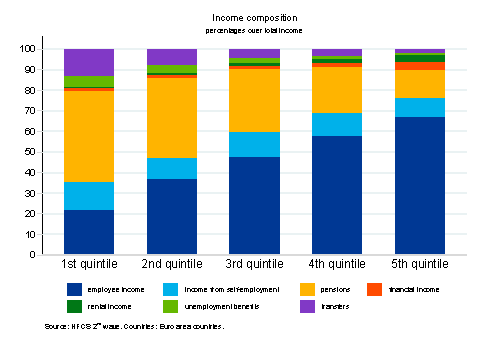
\includegraphics[width=0.66\textwidth]{./figures/incomeComposition_detailed}
\end{center}
\end{figure}

\end{frame}


\begin{frame}\frametitle{\bf Substantial heterogeneity across wealth \hypertarget{WealthSim}{}}

\bi
%\setlength{\itemsep}{2mm}
\item High share of \textbf{\color{ao}main residence} and \textbf{\color{capri} other real estate}
\item Increasing (though moderate) share of \textbf{\color{amber} self-empl business,} \textbf{\color{red} stocks,} \textbf{\color{jgreen} bonds}
\ei
\centering{\footnotesize Composition of total assets}
\vspace*{-2.5mm}
\begin{figure}
\begin{center}
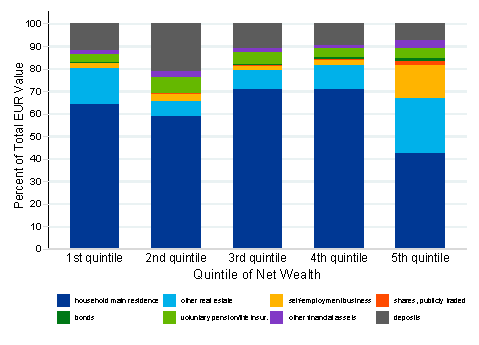
\includegraphics[width=0.66\textwidth]{./figures/wealthCompositionDetailed} %irf_IR irf_fin
\end{center}
\end{figure}
\end{frame}


\begin{frame}\frametitle{\bf Effects of MP on income and wealth components\\ \normalsize{Lenza and Slacalek (2018)}}

%Lenza and Slacalek (2018)\\[2mm]
\jemph{Step 1: Aggregate data --- Separate effects of MP from other factors}
\renewcommand*{\theenumi}{\alph{enumi}}
\begin{enumerate}
\item Estimate \jbemph{VAR} with aggregate unempl \&\ asset prices
\item Quantify \jbemph{impulse responses} of asset prices / unemployment to MP\\[5mm] {}
\end{enumerate}
\jemph{Step 2: Household-level data --- Investigate heterogeneity across households}
\begin{enumerate}
\setcounter{enumi}{2}
\item Transpose IRFs over \jbemph{household-level HFCS data} on wealth, income and their components
\item For employment, use simulation based on probit for employment status
\item Estimate effects of QE on wealth \jbemph{and income} inequality (Gini \dots)
%\item (Implications for transmission of MP to \jbemph{consumption})
\end{enumerate}
\renewcommand*{\theenumii}{\Num{enumi}}

\end{frame}


\begin{frame}\frametitle{\bf Unemployment: Disproportionate decrease for low income}
Impulse: QE $\Rightarrow$ drop in interest rate term spread \jemph{by 30 basis points}
\begin{figure}
\begin{center}
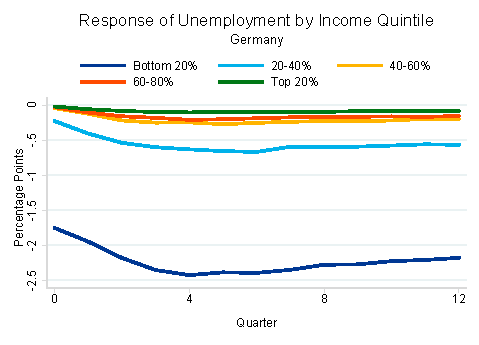
\includegraphics[width=0.38\textwidth]{./figures/UR_chart_DE}
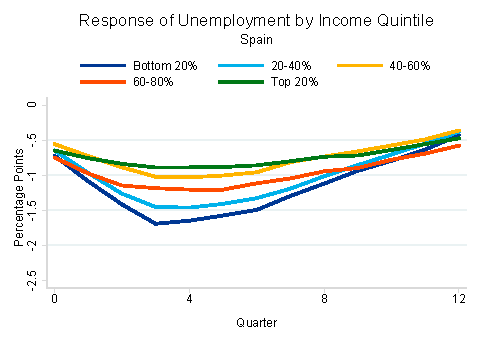
\includegraphics[width=0.38\textwidth]{./figures/UR_chart_ES}\\
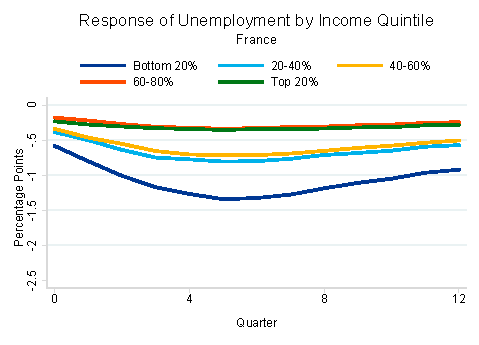
\includegraphics[width=0.38\textwidth]{./figures/UR_chart_FR}
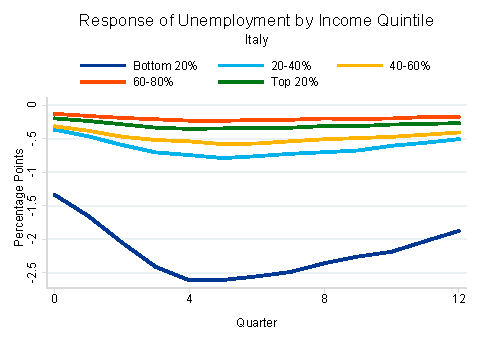
\includegraphics[width=0.38\textwidth]{./figures/UR_chart_IT}
\end{center}
\end{figure}

\end{frame}


\begin{frame}\frametitle{\bf Unemployment}
ES: Unemployed affected in all quintiles b/c distributed more evenly\\
DE, IT: UR strongly skewed toward lowest income quintile
\begin{figure}
\begin{center}
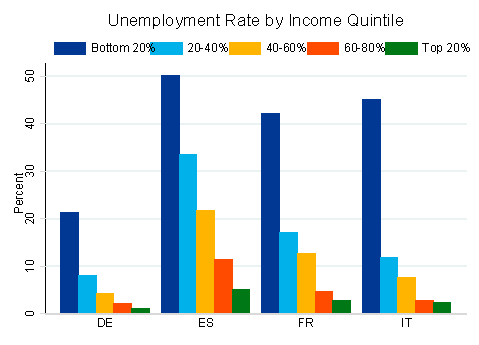
\includegraphics[width=0.7\textwidth]{./figures/URbyIncQuint.pdf}
\end{center}
\end{figure}
\end{frame}


\begin{frame}\frametitle{\bf Income: Larger increases at lower levels}
Unemployment benefits more generous in DE, FR than in ES and \textbf{IT}
\begin{figure}
\begin{center}
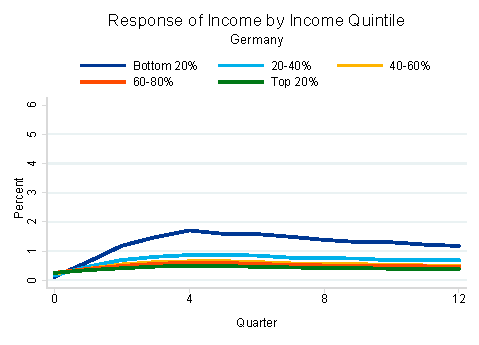
\includegraphics[width=0.38\textwidth]{./figures/di2000_chart_DE}
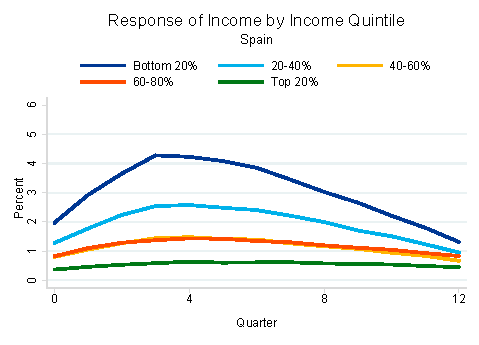
\includegraphics[width=0.38\textwidth]{./figures/di2000_chart_ES}\\
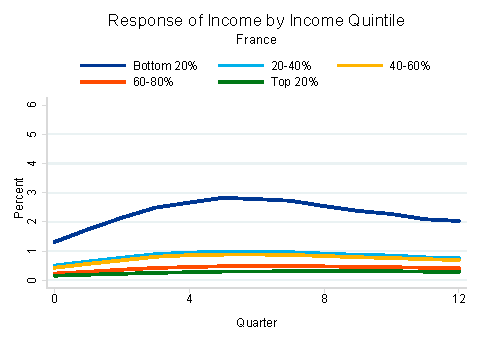
\includegraphics[width=0.38\textwidth]{./figures/di2000_chart_FR}
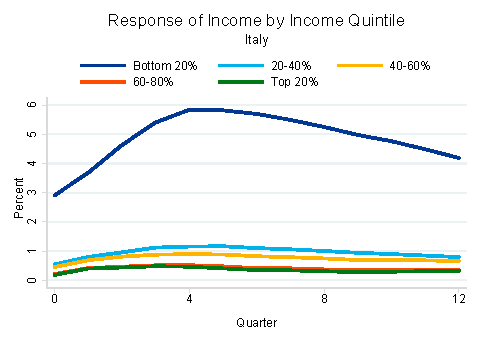
\includegraphics[width=0.38\textwidth]{./figures/di2000_chart_IT}
\end{center}
\end{figure}

\end{frame}


\begin{frame}\frametitle{\bf Reduction of income inequality}
\jbemph{Lower inequality:} Gini for EA goes down from 43.1 to 42.8\\
\jemph{Key importance of extensive margin (Unemp ${}\rightarrow{}$ Emp)}
\begin{figure}
\begin{center}
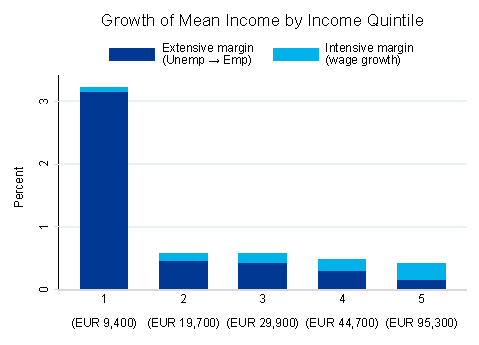
\includegraphics[width=0.7\textwidth]{./figures/meanIncomeByIncQuint_EA_decomp_per4}\\[-2mm]
{\tiny Response of mean income 4 quarters after QE shock. Numbers in brackets: Initial levels of mean gross Hh income. }
\end{center}
\end{figure}

\end{frame}

\begin{frame}\frametitle{\bf Wealth inequality stable \hypertarget{WealthIneq}{}}
\jbemph{Very small effect:} Gini goes down from 68.09 to 68.07\\
\hspace*{32mm}Important to account for house prices \hyperlink{WealthDecomp}{\beamergotobutton{Decomposition}}\\
{\scriptsize $[$Assumes: \jemph{no portfolio rebalancing;} in line with literature on inertia in Hh portfolios (Ameriks, Zeldes, 2004; Bilias et al.\ (2010)$]$}
\begin{figure}
\begin{center}
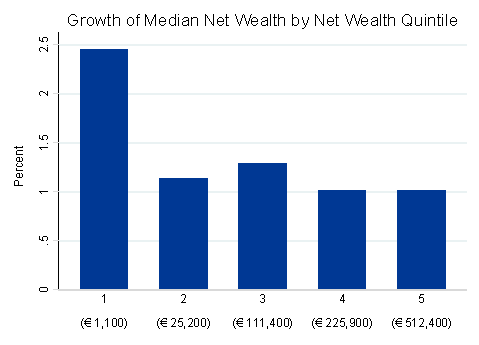
\includegraphics[width=0.6\textwidth]{./figures/medianNetWealthByWquint_EA}\\[-2mm]
{\tiny Response of median net wealth 4 quarters after QE shock. Numbers in brackets: Initial levels of median net wealth.
}
\end{center}
\end{figure}
\end{frame}


\section{Consumption}
\begin{frame}
\bi\setlength{\itemsep}{3mm}
\item Motivation
\item Effects of monetary policy on income and wealth
\item \jbemph{Effects of monetary policy on consumption}
\item Summary
\ei
\end{frame}



\begin{frame}\frametitle{\bf Implications for behavior of consumption \hspace*{\fill} \footnotesize{Ampudia et al.\ (2018)} }


\bi\setlength{\itemsep}{2mm}
\item {Consensus in recent literature on C $[$also HANK; Brinca$\,\&\,$Krusell (2016); \dots$]$:}\\
Many households (25--30\%) are \jemph{constrained} (`hand-to-mouth') 
\pause
\item Constrained households have \jemph{large MPCs:$0.3$--$0.6$}
\pause
\item This presentation so far: \jbemph{Employment of constrained Hhs responsive to MP}
\pause
\item  HANK decomposition \`a\ la Kaplan et al.~(2018), Auclert~(2019)\\[1mm]
Total effect of MP on consumption = Direct effects + Indirect (GE) effect
{\small
$$
\frac{\Delta C}{C}=\underbrace{\overbrace{MPC\cdot\frac{\text{\scriptsize{Interest Exposure}}}{C}\cdot\Delta R}^{\text{(Net) Interest Rate-Sensitive Assets}}-\overbrace{\sigma\cdot(1-MPC)\cdot\Delta R}^{\text{Intertemporal Substitution}}}_{\text{\jemph{Direct Effects}}}+\underbrace{\overbrace{MPC\cdot\frac{Y}{C}\cdot\frac{\Delta Y}{Y}}^{\text{Reaction of Income to $\Delta R$}}}_{\text{\jemph{Indirect Effect}}}
$$
}
\pause
%\item All effects heterogeneous across households depending on income/wealth composition, labor status, \dots
 \item \jemph{MPC${}\times\frac{\Delta Y}{Y}$ matters for strength of \jbemph{indirect channel of monetary transmission} (GE/aggregate demand) }\\
% \item Other effects (via wealth effects, net nominal positions) probably less important in EA
\ei


\end{frame}



\begin{frame}\frametitle{\bf HANK decomposition of effects of monetary policy on C}
\vspace*{-2.5mm}
\footnotesize
$$
\frac{\Delta C}{C}=\underbrace{\overbrace{MPC\cdot\frac{\text{\scriptsize{Interest Exposure}}}{C}\cdot\Delta R}^{\text{(Net) Interest Rate-Sensitive Assets}}-\overbrace{\sigma\cdot(1-MPC)\cdot\Delta R}^{\text{Intertemporal Substitution}}}_{\text{\jemph{Direct Effects}}}+\underbrace{\overbrace{MPC\cdot\frac{Y}{C}\cdot\frac{\Delta Y}{Y}}^{\text{Reaction of Income to $\Delta R$}}}_{\text{\jemph{Indirect Effect}}}
$$
\small
\jbemph{Effects of 100 bp cut in short-term $R$ on C} in DE and ES
\begin{figure}
\begin{center}
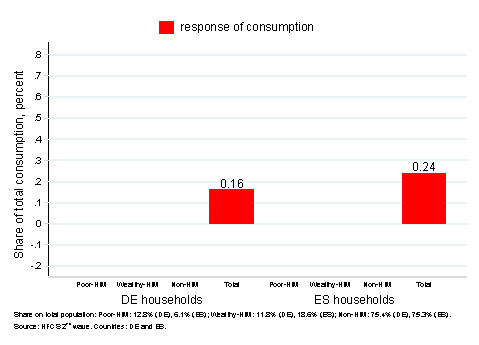
\includegraphics[width=0.6\textwidth]{./figures/cDecomp1.pdf}
\end{center}
\end{figure}
\end{frame}



\begin{frame}\frametitle{\bf HANK decomposition of effects of monetary policy on C}
\vspace*{-2.5mm}
\footnotesize
$$
\frac{\Delta C}{C}=\underbrace{\overbrace{MPC\cdot\frac{\text{\scriptsize{Interest Exposure}}}{C}\cdot\Delta R}^{\text{(Net) Interest Rate-Sensitive Assets}}-\overbrace{\sigma\cdot(1-MPC)\cdot\Delta R}^{\text{Intertemporal Substitution}}}_{\text{\jemph{Direct Effects}}}+\underbrace{\overbrace{MPC\cdot\frac{Y}{C}\cdot\frac{\Delta Y}{Y}}^{\text{Reaction of Income to $\Delta R$}}}_{\text{\jemph{Indirect Effect}}}
$$
\small
\jbemph{Effects of 100 bp cut in short-term $R$ on C} in DE and ES, by hand-to-mouth status 
\begin{figure}
\begin{center}
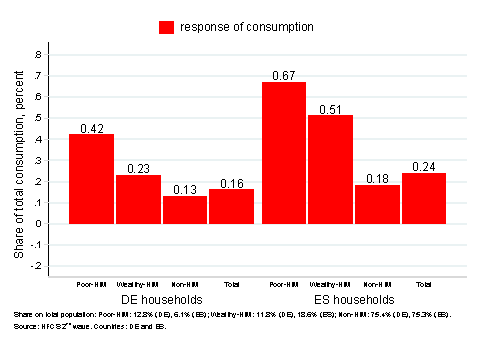
\includegraphics[width=0.6\textwidth]{./figures/cDecomp2.pdf}
\end{center}
\end{figure}
\end{frame}



\begin{frame}\frametitle{\bf HANK decomposition of effects of monetary policy on C}
\vspace*{-2.5mm}
\footnotesize
$$
\frac{\Delta C}{C}=\underbrace{\overbrace{MPC\cdot\frac{\text{\scriptsize{Interest Exposure}}}{C}\cdot\Delta R}^{\text{(Net) Interest Rate-Sensitive Assets}}-\overbrace{\sigma\cdot(1-MPC)\cdot\Delta R}^{\text{Intertemporal Substitution}}}_{\text{\jemph{Direct Effects}}}+\underbrace{\overbrace{MPC\cdot\frac{Y}{C}\cdot\frac{\Delta Y}{Y}}^{\text{Reaction of Income to $\Delta R$}}}_{\text{\jemph{Indirect Effect}}}
$$
\small
\jbemph{Effects of 100 bp cut in short-term $R$ on C} in DE and ES, by hand-to-mouth status 
\begin{figure}
\begin{center}
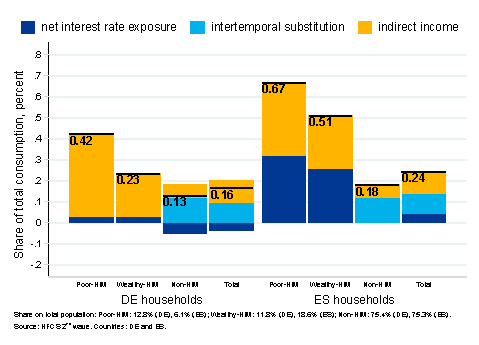
\includegraphics[width=0.6\textwidth]{./figures/cDecomp3.pdf}
\end{center}
\end{figure}
\end{frame}



\begin{frame}
\bi\setlength{\itemsep}{3mm}
\item Motivation
\item Effects of monetary policy on income and wealth
\item Effects of monetary policy on consumption
\item \jbemph{Summary}
\ei
\end{frame}


\section{Summary}
\begin{frame}\frametitle{\bf Summary}
\jbemph{\large Monetary policy:}\\
\bi\setlength{\itemsep}{3mm}
\item \jemph{Reduces income inequality}
\item Has substantial impact on employment / income in bottom tail
\item Effect on wealth inequality small
\item \jemph{Consumption:}\\ Indirect (GE) effect important, especially for constrained households
\ei
\pause

\vspace*{2.5mm}
\jbemph{\large Important to account for (the substantial) household heterogeneity}

\end{frame}


%%%%%%%%%%%%%%%%%%%%%%%%%%%%%%%%%%%%%%%%%%%%%%%%%%%%%%%%%%%%%%%%%%%%%%%%%%%%%%
%%%%%%%%%%%%%%%%%%%%%%%%%%%%%%%%%%%%%%%%%%%%%%%%%%%%%%%%%%%%%%%%%%%%%%%%%%%%%%

\section{Background slides}
\begin{frame}

\begin{center}
\Large
\jbemph{Background slides}
\end{center}

\end{frame}


%\section{Literature}
\begin{frame}\frametitle{\bf Existing literature}
\bi
\setlength{\itemsep}{2mm}
\item \jbemph{Macro effects of nonstandard MP---VARs:}\\
{\footnotesize Baumeister and Benati (IJCB, 2013); Altavilla et al.\ (IJCB, 2016); \dots}
\item \jbemph{VARs with income / consumption Ginis:}\\
{\footnotesize  Coibion et al.\ (JME, 2017); Mumtaz and Theophilopoulou (EER, 2017)}
\bi
\item No \jemph{wealth} inequality, don't estimate effects of \jemph{nonstandard MP}
\ei
\item \jbemph{Household wealth portfolios, inflation and asset prices:}\\
{\footnotesize  Doepke and Schneider (JPE, 2006); Adam and Zhu (JEEA, 2016); Adam and Tzamourani (EER, 2016); Doepke et al.\ (2016)}
\bi
\item Assume \jemph{hypothetical scenarios,} eg ``10\%\ increase in price level''
\ei
\item \jbemph{Model-based simulations:}\\
{\footnotesize Casiraghi et al.\ (2018) [BdI]; Bunn et al.\ (2018) [BoE]}
\bi
\item More calibrated than estimated
\ei
\ei

\bi
\item \jbemph{So far little quantitative, estimated work on effects of nonstandard MP on inequality}
\ei

\end{frame}


\begin{frame}\frametitle{\bf Gaps in existing work }
Not much work with micro data on:\\
\bi
\setlength{\itemsep}{2mm}
\item House prices / housing wealth
\item Employment effects / income inequality
\item Little estimated quantitative evidence in general
\item Even less on non-standard MP
\ei

\end{frame}


%\section{VAR}
\begin{frame}\frametitle{\bf\large Step 1: Multi-country VAR to estimate aggr effects of QE}

\vspace*{-11.5mm}
\begin{align*}
y{_t}&=C+B{_1}  y_{t-1}+\cdots+B{_p}  y_{t-p}+\epsilon_{t}\\
\epsilon_{t}&=N(0,\Sigma)
\end{align*}
\vspace*{-7.5mm}
\bi
\setlength{\itemsep}{2mm}
\item Mix of EA and country-level variables; \jemph{4 countries: DE, FR, IT, ES}
\item $\Rightarrow$ \jbemph{Common MP ${}+{}$ country heterogeneity in responses}
\item Variables $y_t$:
\bi
\item \jemph{Country-specific:} real GDP, GDP defl, \jbemph{wages, unempl, house prices}
\item \jemph{EA:} short- and long-term interest rates, \jbemph{stock prices}
\item \jemph{US:} GDP, short-term interest rates
\ei
\item Large dimension $\Rightarrow$ \jbemph{Bayesian estimation} (Litterman, 1979; Giannone, Lenza and Primiceri, 2015)
\item Quarterly data: 1999Q1--2016Q4, $p=5$ lags
\ei
\end{frame}



\begin{frame}\frametitle{\bf\large VAR: Identification \`a la Baumeister and Benati (2013)}
\begin{enumerate}
\setlength{\itemsep}{2mm}
\item Identify exogenous asset purchase shock with \jbemph{zero and sign restrictions} (Arias et al., 2017)\\[2mm]
\jbemph{Sign restrictions}---Expansionary \jbemph{QE (APP) shock} on impact:
\bi
\item Decreases term IR spread
\item Increases real GDP
\ei
\item \jbemph{Offset response of EA policy rate} via series of standard MP shocks
\bi
\item \dots because standard MP did not react to offset effects of asset purchases (policy rate remained at lower bound)
\ei
\item Standard MP shock identified via standard zero (Choleski) restrictions
\end{enumerate}

\end{frame}



\begin{frame}\frametitle{\bf Impulse responses---QE shock}
\bi
\item Size of QE shock to term spread scaled to \jbemph{30 bp} on impact\\
In line with Altavilla et al.\ (2015) and Andrade et al.\ (2016)
\ei
\begin{figure}
\begin{center}
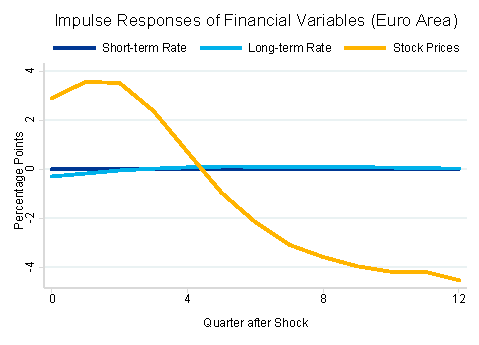
\includegraphics[width=0.7\textwidth]{./figures/irf_fin} %irf_IR irf_fin
\end{center}
\end{figure}

\end{frame}



\begin{frame}\frametitle{\bf Impulse responses of key aggregate variables}
\bi
\item UR, HP responses stronger in ES, milder in DE
\item Link to ARM, mortgage / labor market institutions?
\ei
\begin{figure}
\begin{center}
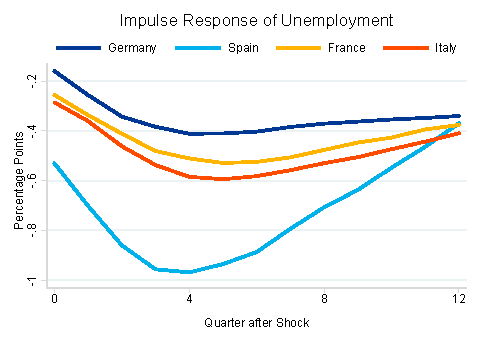
\includegraphics[width=0.5\textwidth]{./figures/irf_UR}
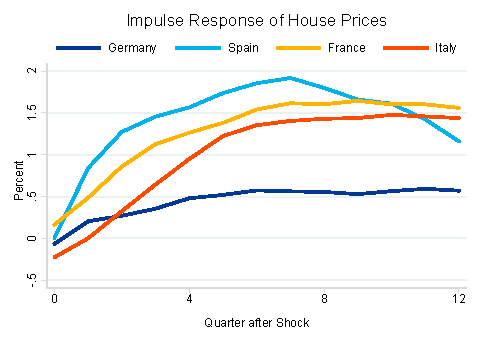
\includegraphics[width=0.5\textwidth]{./figures/irf_HP}
\end{center}
\end{figure}
\bi
\item Stock prices included at EA level
\ei
\end{frame}


%\section{HFCS estimation}

%\subsection{U Sim}
\begin{frame}\frametitle{\bf\large Unemployment simulation---Extensive margin {\scriptsize$[$Ampudia et al.\ (2016)$]$}\\
\small Some unemployed become employed and receive wage given by Heckman}
%{\small Unemployment simulation following Ampudia et al.\ (2016)}
\begin{block}{\jbemph{\small 1.\ Probit for employment status}}
\small
\bi
\setlength{\itemsep}{0mm}
\item Country ($c$)-specific at individual level (not Hh): $$\Pr(Y=1|X=x) = \Phi(x_{c,i}'\hat\beta_c)$$
$Y$ empl status, $X$ demographics (gender, edctn, age, mar status, chldrn)
\item Collect fitted values $\hat Y_{c,i}$; draw \jemph{uniformly distributed} shock $\epsilon_{c,i}$
\item \jemph{If $\epsilon_{c,i}$ sufficiently below $\hat Y_{c,i}$ $\Rightarrow$ unempl individual $i$ becomes employed}
\item \jemph{$\sum$ newly employed people ${}={}$ aggregate decline in unempl implied by VAR}
\item Repeat many times for different draws of $\epsilon_{c,i}$, average across sims
\ei
\end{block}

\begin{block}{\jbemph{\small 2.\ Heckman selection model to estimate unobserved wages}}
\small
\bi
\item \jemph{Income of the newly employed \jbemph{increases} as implied by Heckman:}\\[0mm]
They receive wage instead of (lower) unempl benefits\\
{\scriptsize{Exclusion restrictions: marital status, children}}
\ei
\end{block}

\end{frame}

%\section{Results}

\begin{frame}\frametitle{\bf Robustness \hypertarget{Robust}{}}

\bi
\item \jemph{Local linear projections (Jord\`a, 2005):}\\ How do other variables respond to QE shock?
\bi
\item  Holdings of wealth components (flow of funds) \hyperlink{FoF}{\beamergotobutton{}}
\item ES local house prices \hyperlink{ESlocalHP}{\beamergotobutton{}}
\item ES local house prices: IRF vs level \hyperlink{ESlocalHPlevel}{\beamergotobutton{}}
\item Profits / financial income \hyperlink{finInc}{\beamergotobutton{}}
\ei
\item Uniform employment probability \hyperlink{UniformEmpProb}{\beamergotobutton{}}
\item Same VAR response in all countries \hyperlink{SameXC}{\beamergotobutton{}}
\item Financial income $\uparrow$ by 5\% \hyperlink{FinInc}{\beamergotobutton{}}
\item Portfolio rebalancing---some trading in stocks:\\ Buy 15\%\ of your stock holdings \hyperlink{StockBoost}{\beamergotobutton{}}
\ei
\end{frame}



%\section{Implications}



\begin{comment}
\begin{frame}\frametitle{\bf\normalsize Popular hypothesis: Asset purchases boost wealth inequality }
\bi
\item<1-> But what about effects of APP on house prices?
\item<2-> And what about employment effects / income inequality?
\item<2-> Little quantitative evidence in general
\begin{figure}
\begin{center}
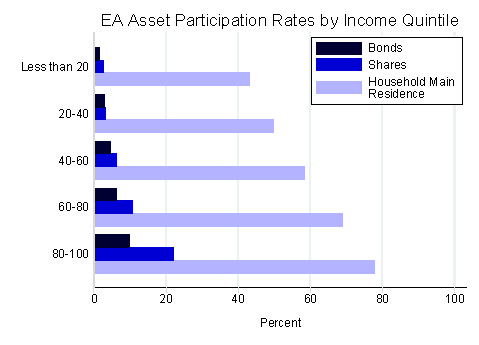
\includegraphics[width=.75\textwidth]{./figures/fAssetParticipationByIncome}
\end{center}
\end{figure}
\ei

\end{frame}
\end{comment}





\begin{frame}\frametitle{\bf Modelling response of wealth and income components to QE \hypertarget{DetailedWealth}{}
\hyperlink{WealthSim}{\beamergotobutton{Back}}
}

\begin{figure}
\begin{center}
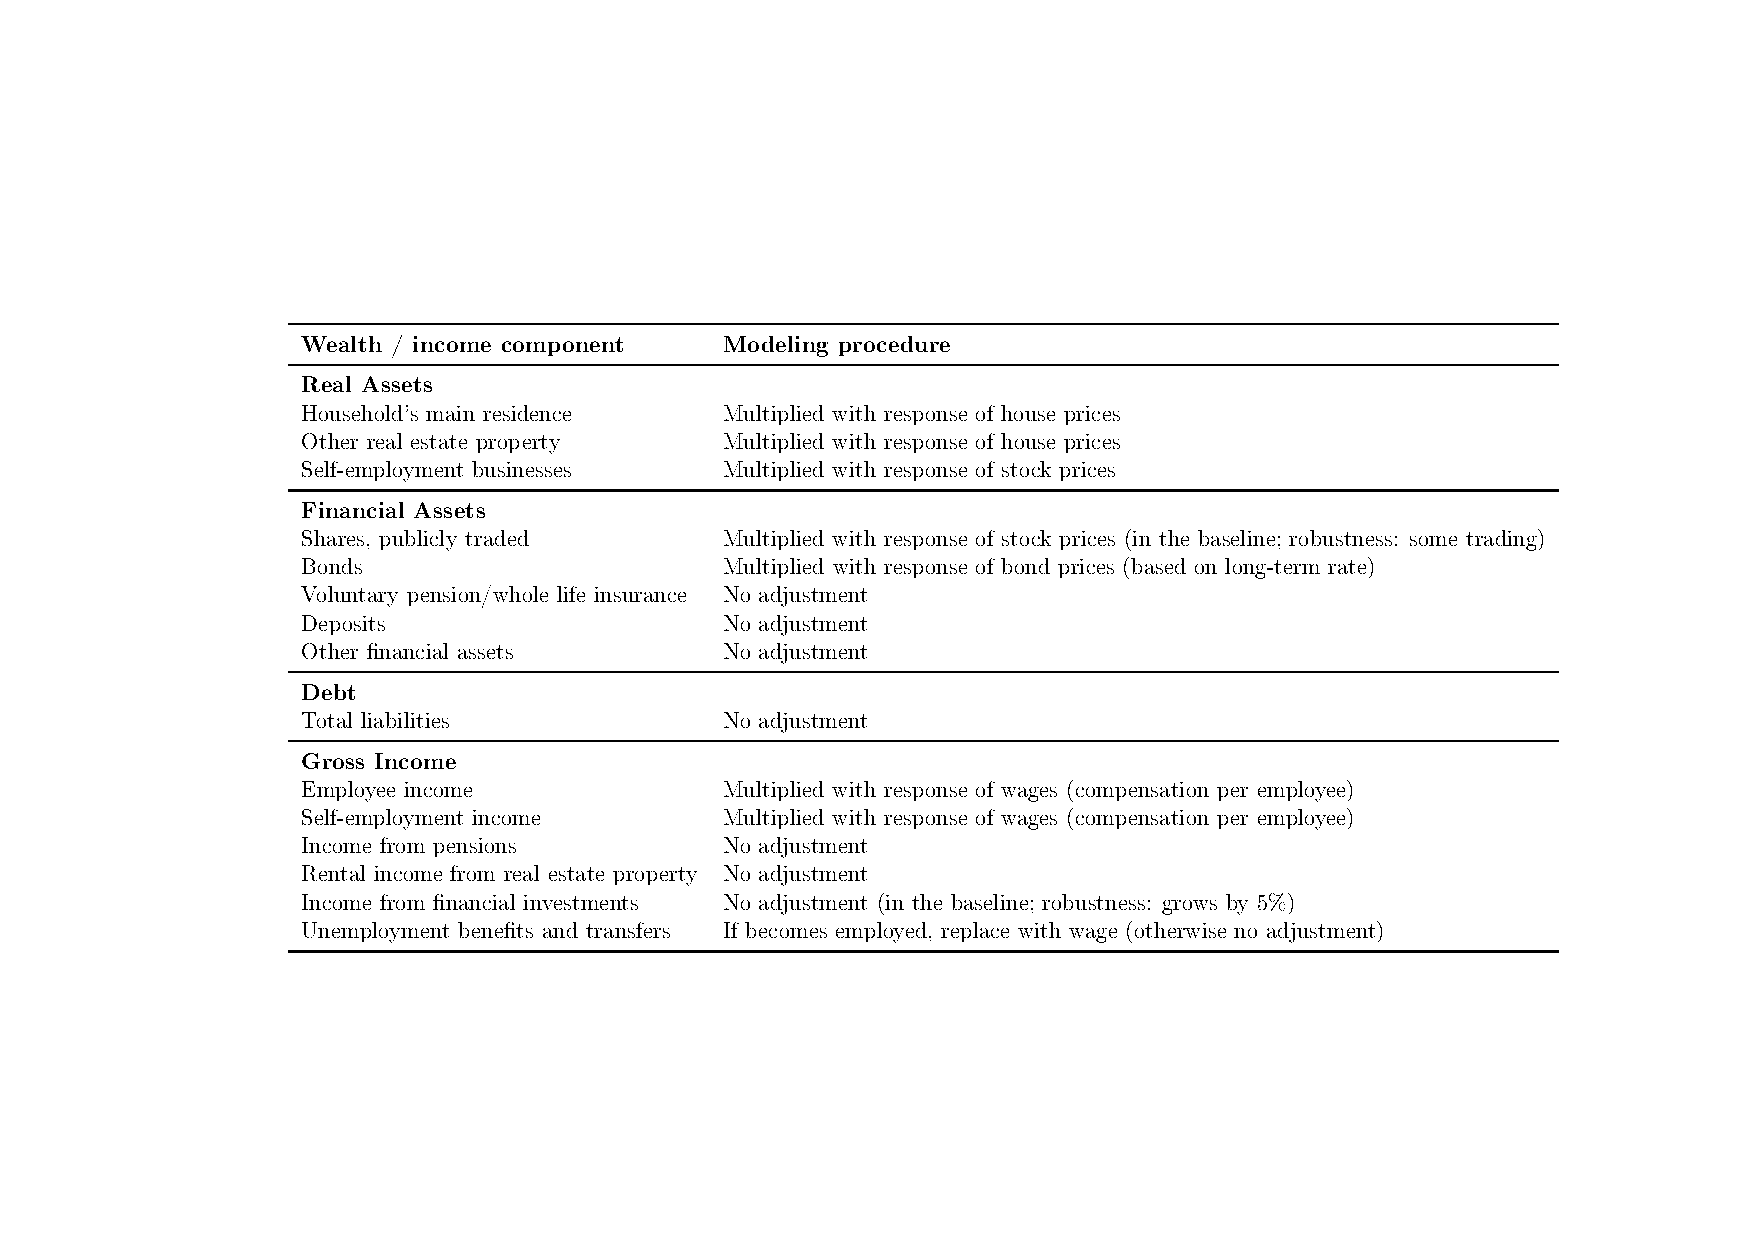
\includegraphics[width=1\textwidth]{./figures/wealthSimulation}
\end{center}
\end{figure}

\end{frame}



\begin{frame}\frametitle{\bf Impact of QE on long-term IR---Literature review}
\begin{figure}
\begin{center}
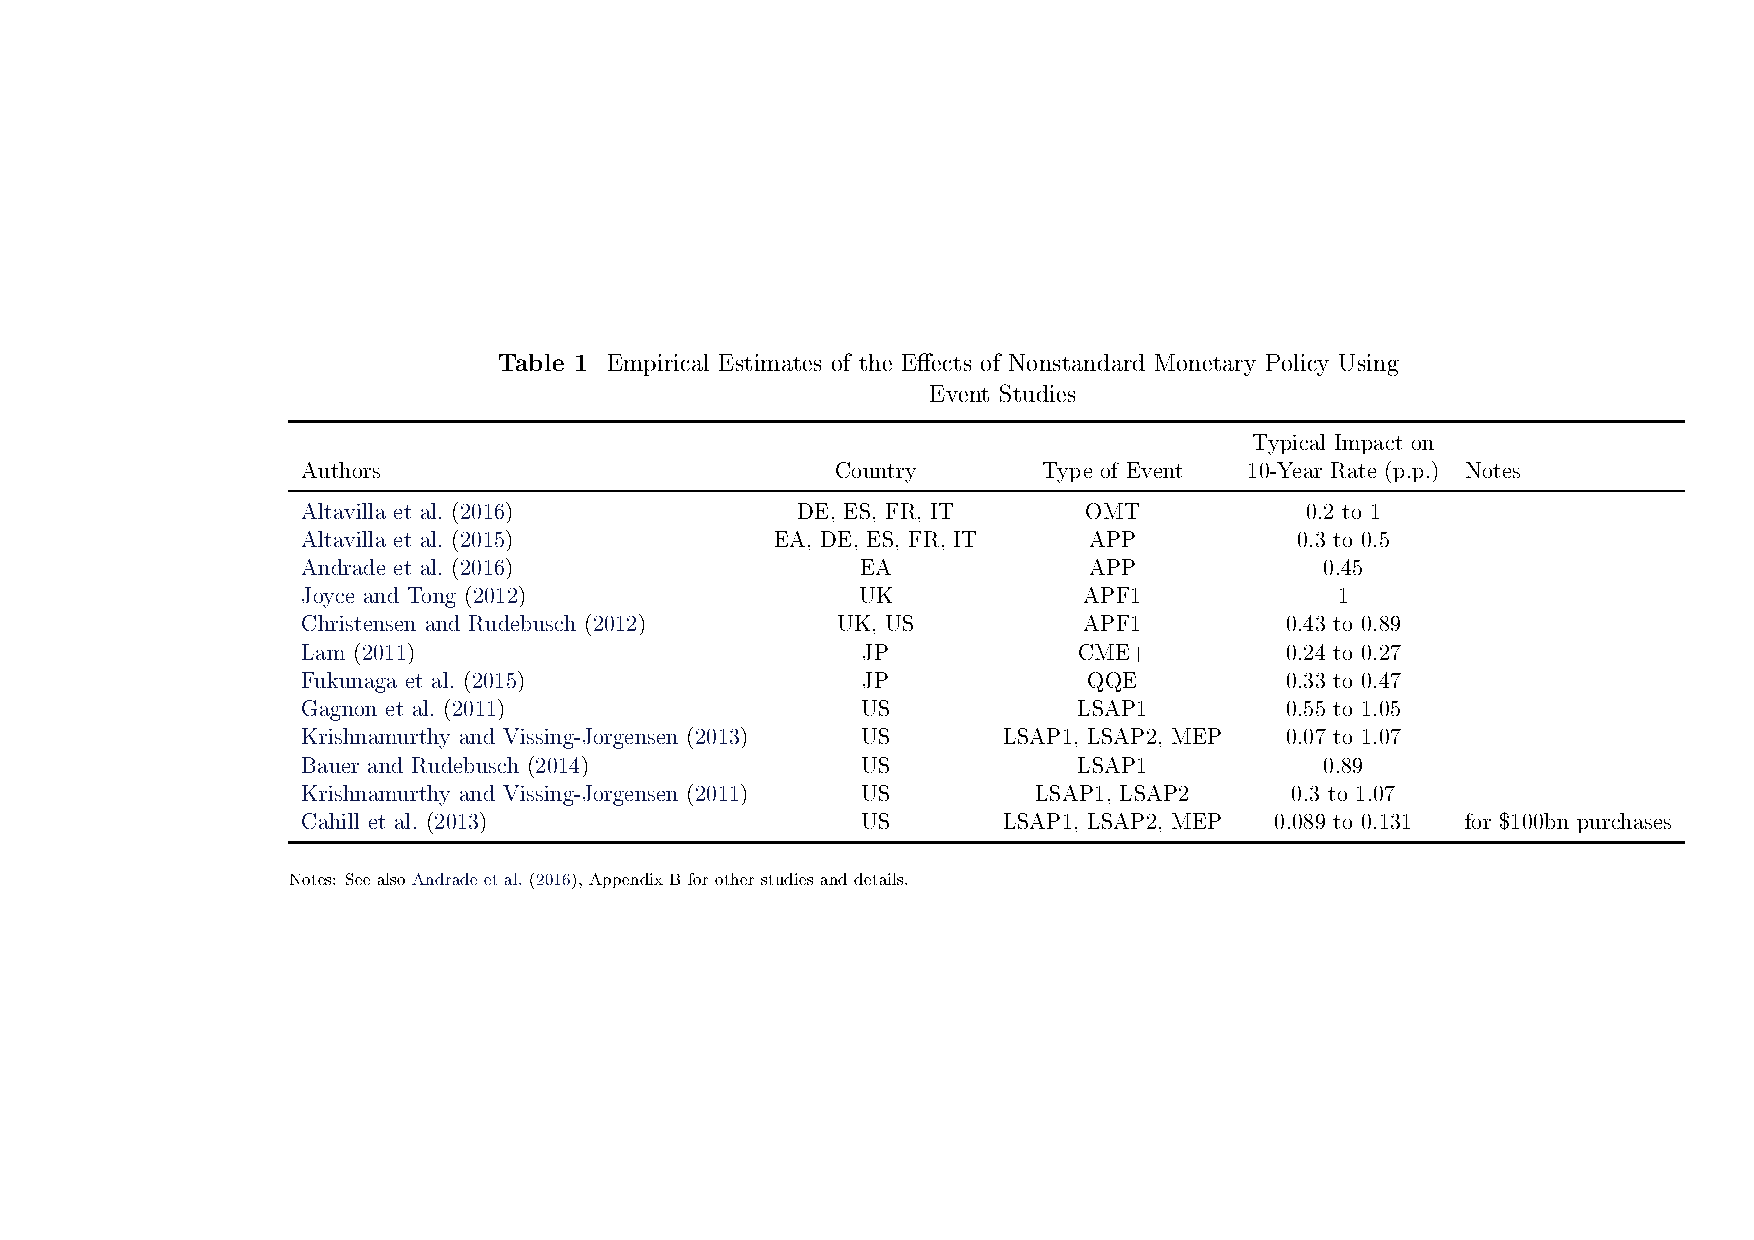
\includegraphics[width=1\textwidth]{./figures/fLitRevAPPsize}
\end{center}
\end{figure}

\end{frame}



\begin{frame}\frametitle{\bf Impulse responses of aggregate variables}
\begin{figure}
\begin{center}
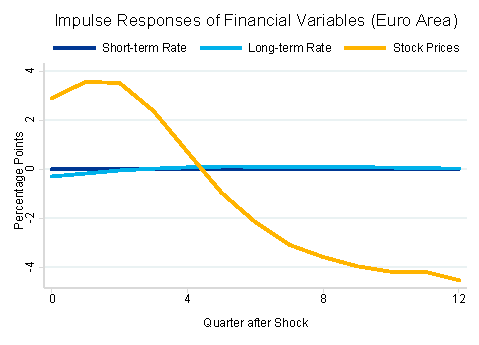
\includegraphics[width=0.45\textwidth]{./figures/irf_fin}
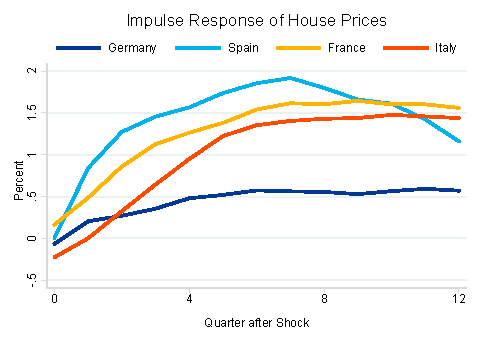
\includegraphics[width=0.45\textwidth]{./figures/irf_HP}\\
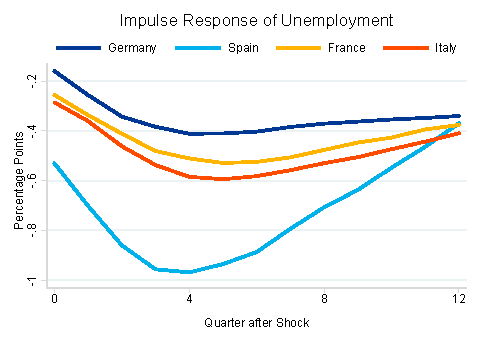
\includegraphics[width=0.45\textwidth]{./figures/irf_UR}
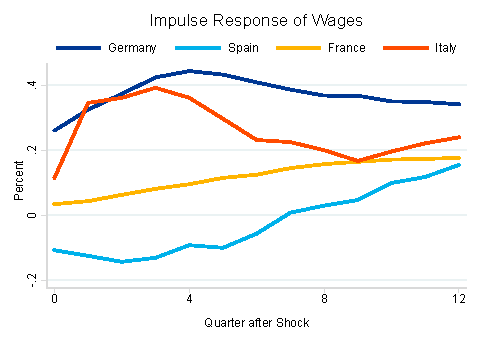
\includegraphics[width=0.45\textwidth]{./figures/irf_W}
\end{center}
\end{figure}

\end{frame}


\begin{comment}
\begin{frame}\frametitle{\bf Impulse responses 4 quarters after shock}
Substantial heterogeneity across countries
\begin{figure}
\begin{center}
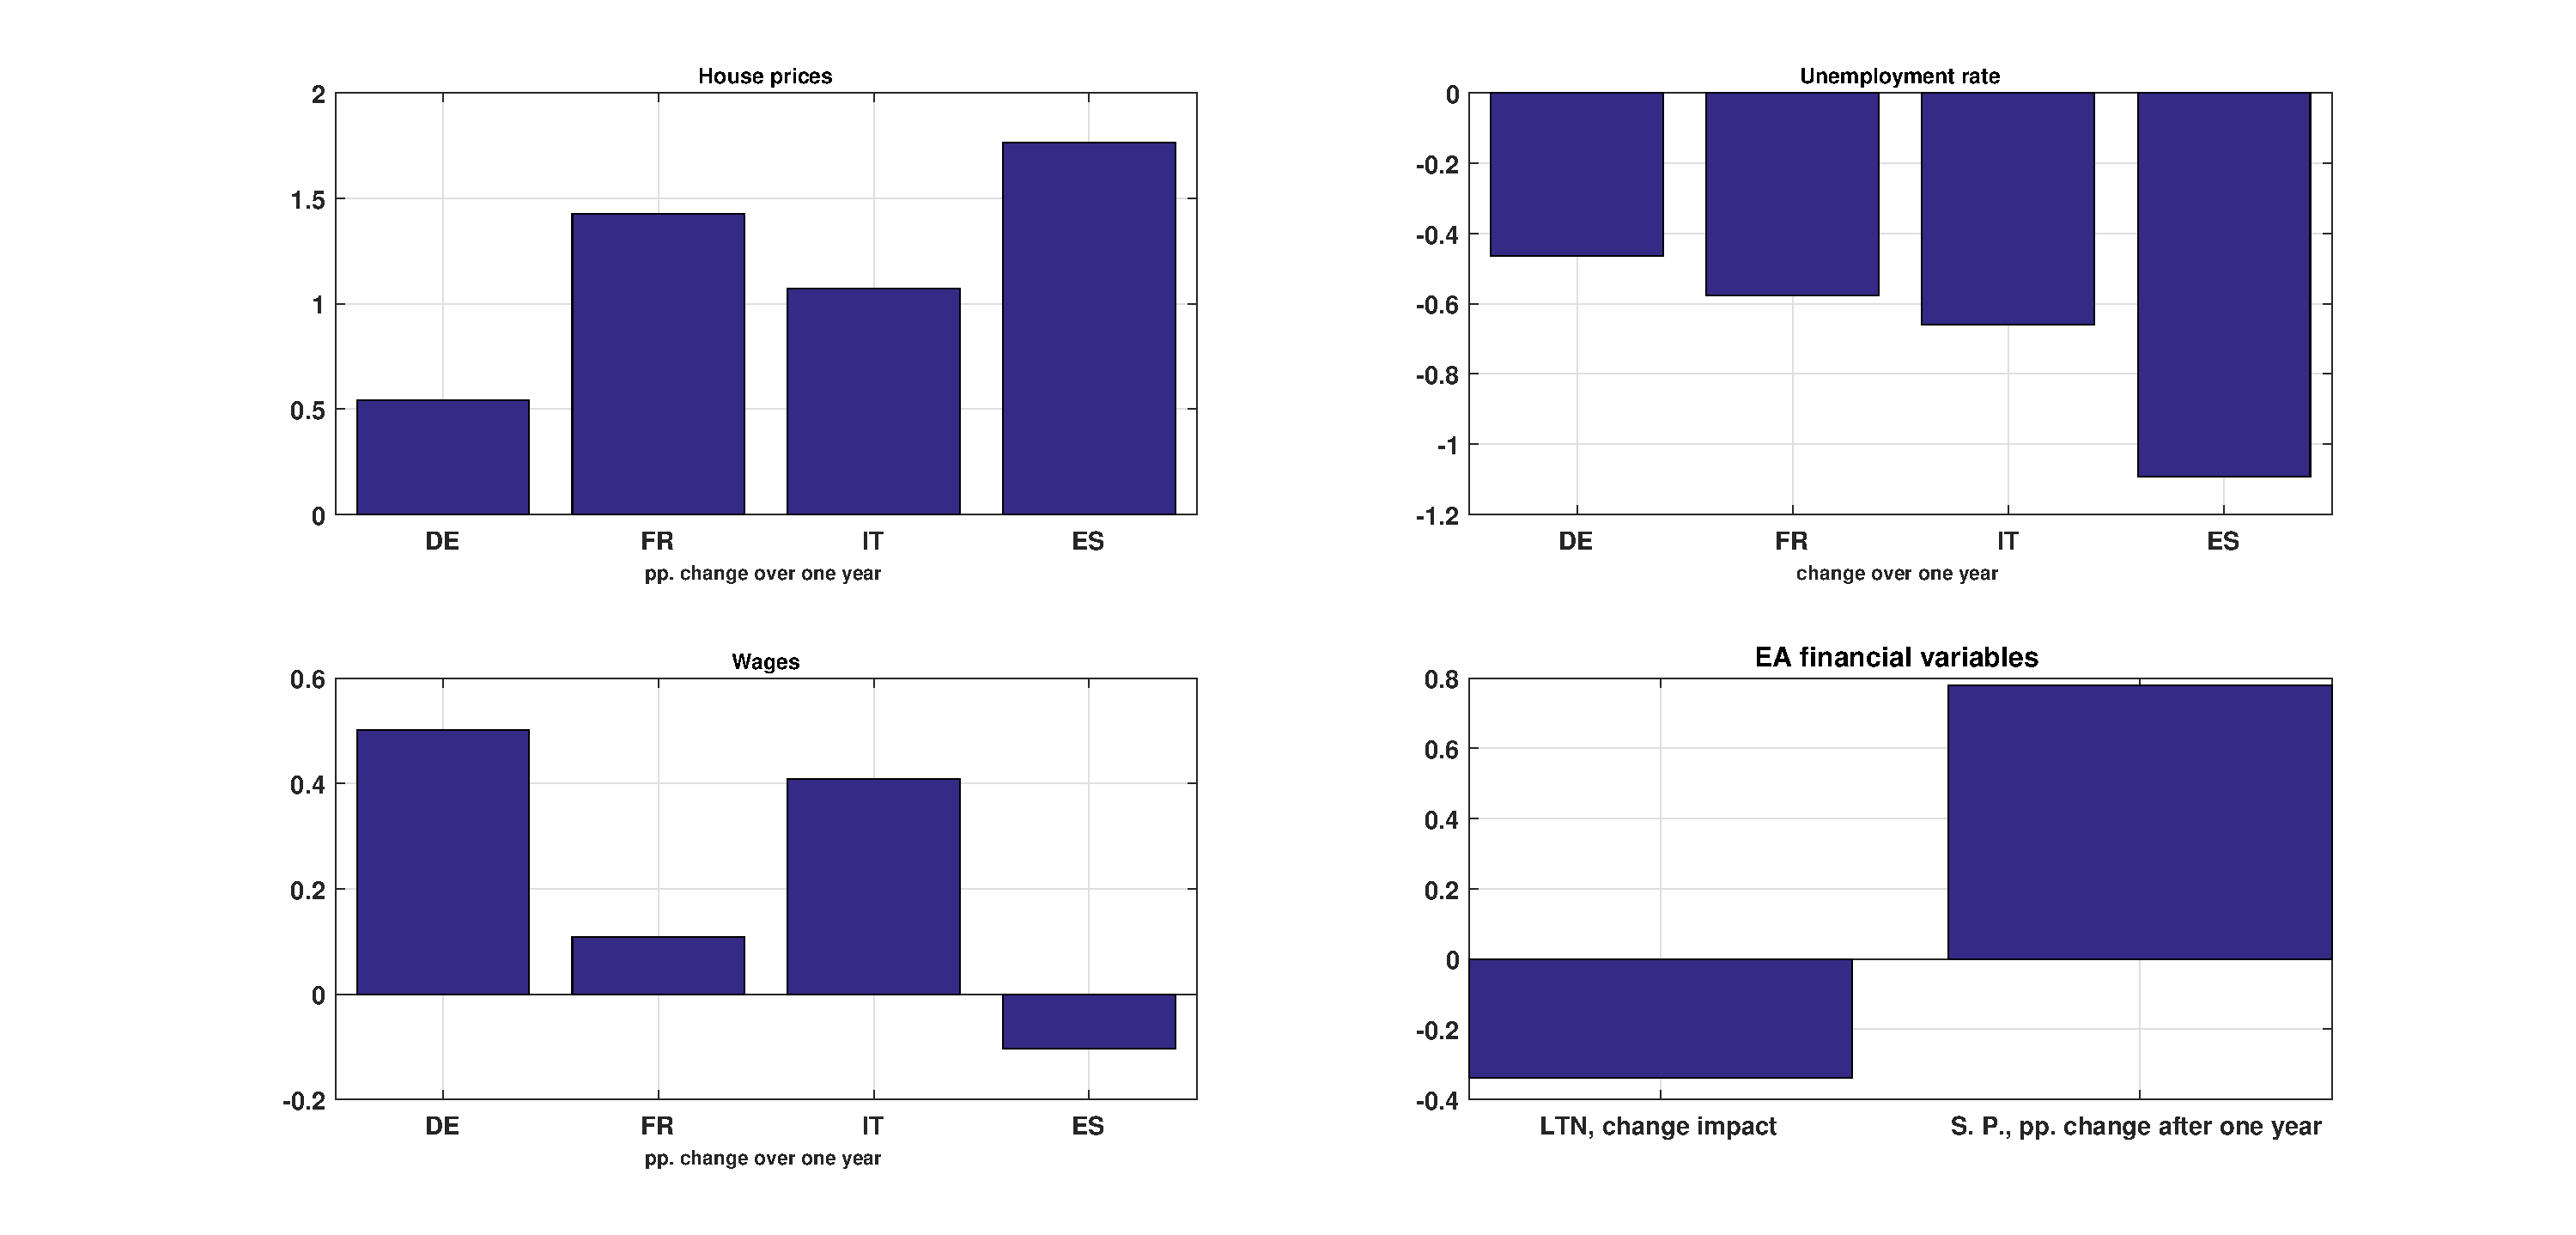
\includegraphics[width=1\textwidth]{./figures/figureIRFs_cut1Y_all}
\end{center}
\end{figure}

\end{frame}
\end{comment}

\begin{frame}\frametitle{\bf EA unemployment}
\jbemph{Disproportionate decrease for low income}

\begin{figure}
\begin{center}
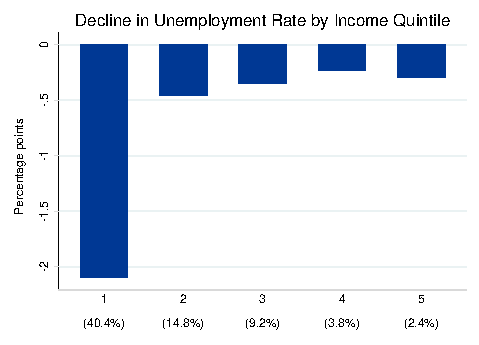
\includegraphics[width=0.8\textwidth]{./figures/urChangeByIncQuint_EA.pdf}
\end{center}
\end{figure}
\end{frame}




\begin{frame}\frametitle{\bf Decomposition of changes in net wealth  \hypertarget{WealthDecomp}{}}
Key role of housing \hyperlink{WealthIneq}{\beamergotobutton{Back}}
\begin{figure}
\begin{center}
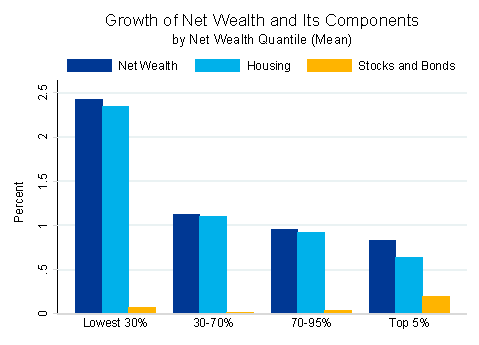
\includegraphics[width=0.7\textwidth]{./figures/wealthDecomp}\\
{\scriptsize Response of mean net wealth and its components 4 quarters after QE shock. }
\end{center}
\end{figure}

\end{frame}



\begin{frame}\frametitle{\bf Net wealth}

{\scriptsize Caveat:  Some increase in wealth above P90, but transitory (see IRF for stock prices)\\
Lower percentiles: Role of leverage}
\begin{figure}
\begin{center}
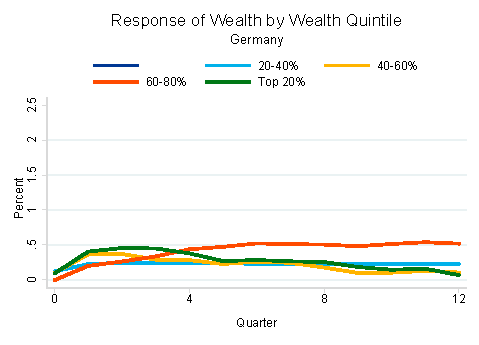
\includegraphics[width=0.40\textwidth]{./figures/dn3001_chart_DE}
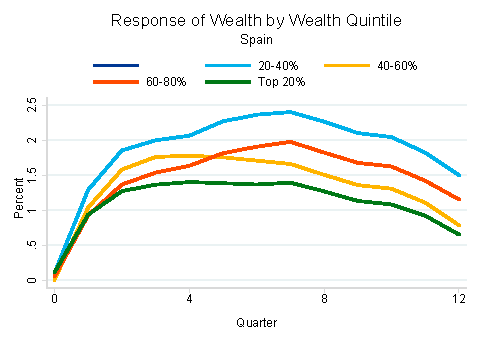
\includegraphics[width=0.40\textwidth]{./figures/dn3001_chart_ES}\\
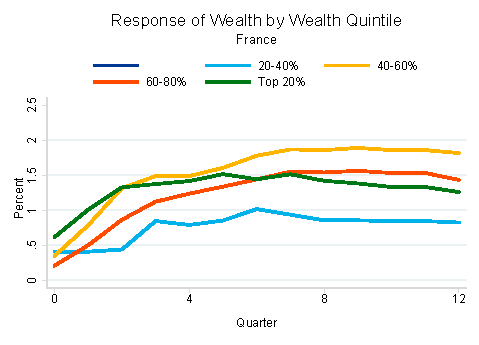
\includegraphics[width=0.40\textwidth]{./figures/dn3001_chart_FR}
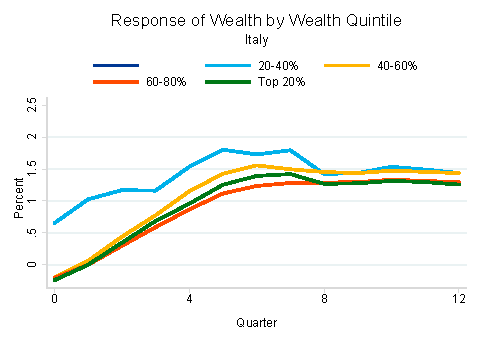
\includegraphics[width=0.40\textwidth]{./figures/dn3001_chart_IT}
\end{center}
\end{figure}
\end{frame}



\begin{frame}\frametitle{\bf Local linear projection:  \\ {\large ES holdings of wealth components (flow of funds) } \hyperlink{Robust}{\beamergotobutton{Back}} \hypertarget{FoF}{}}
Total fin assets $\uparrow\approx5$--$10\%$; stocks $\uparrow$ by a lot ($\approx15\%$), debt $\downarrow$ a bit
\vspace*{-2mm}
\begin{figure}
\begin{center}
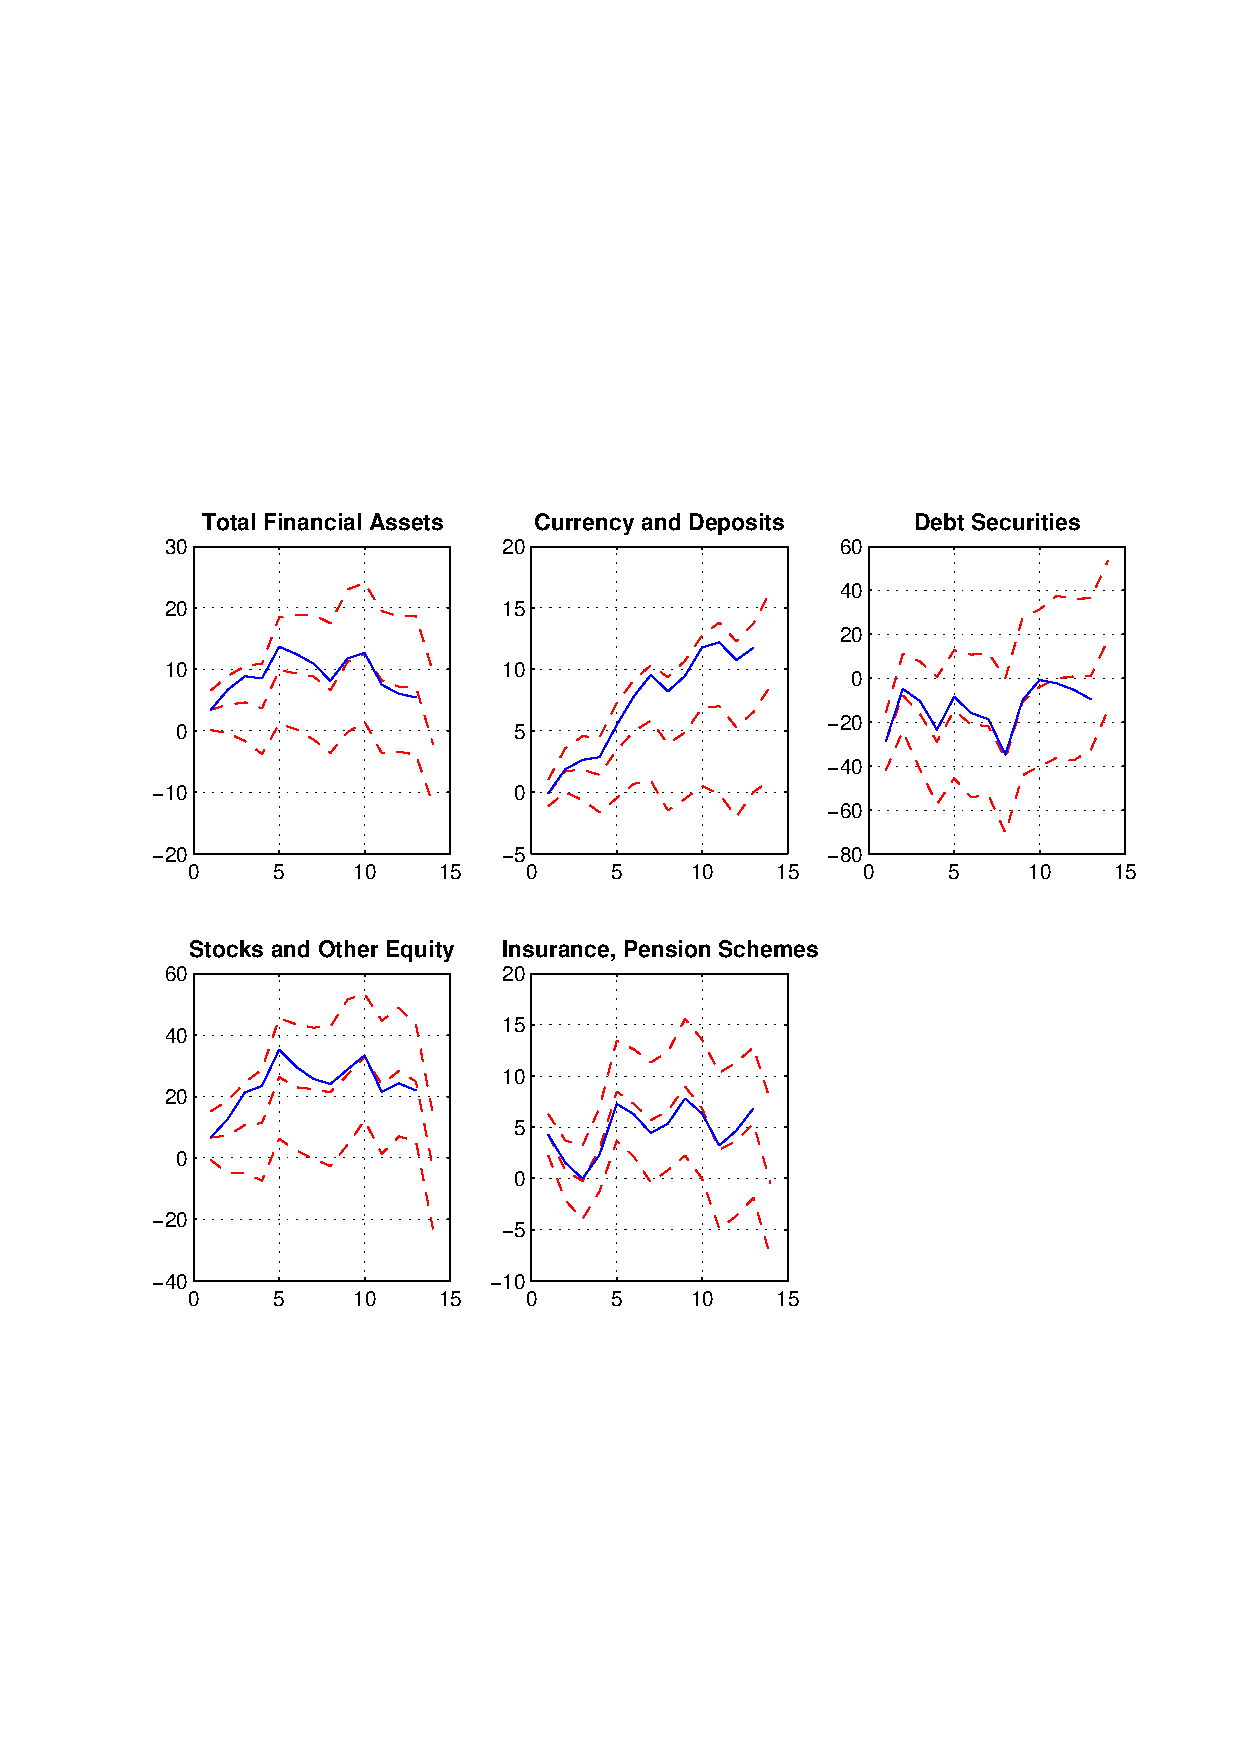
\includegraphics[width=0.7\textwidth]{./figures/fFof_ES}\\
%{\scriptsize Numbers in brackets: Initial levels of mean gross Hh income. }
\end{center}
\end{figure}

\end{frame}



\begin{frame}\frametitle{\bf Local linear projection:   ES regional house prices \hyperlink{Robust}{\beamergotobutton{Back}} \hypertarget{ESlocalHP}{}}
Some, but not overwhelming heterogeneity
\vspace*{-5mm}
\begin{figure}
\begin{center}
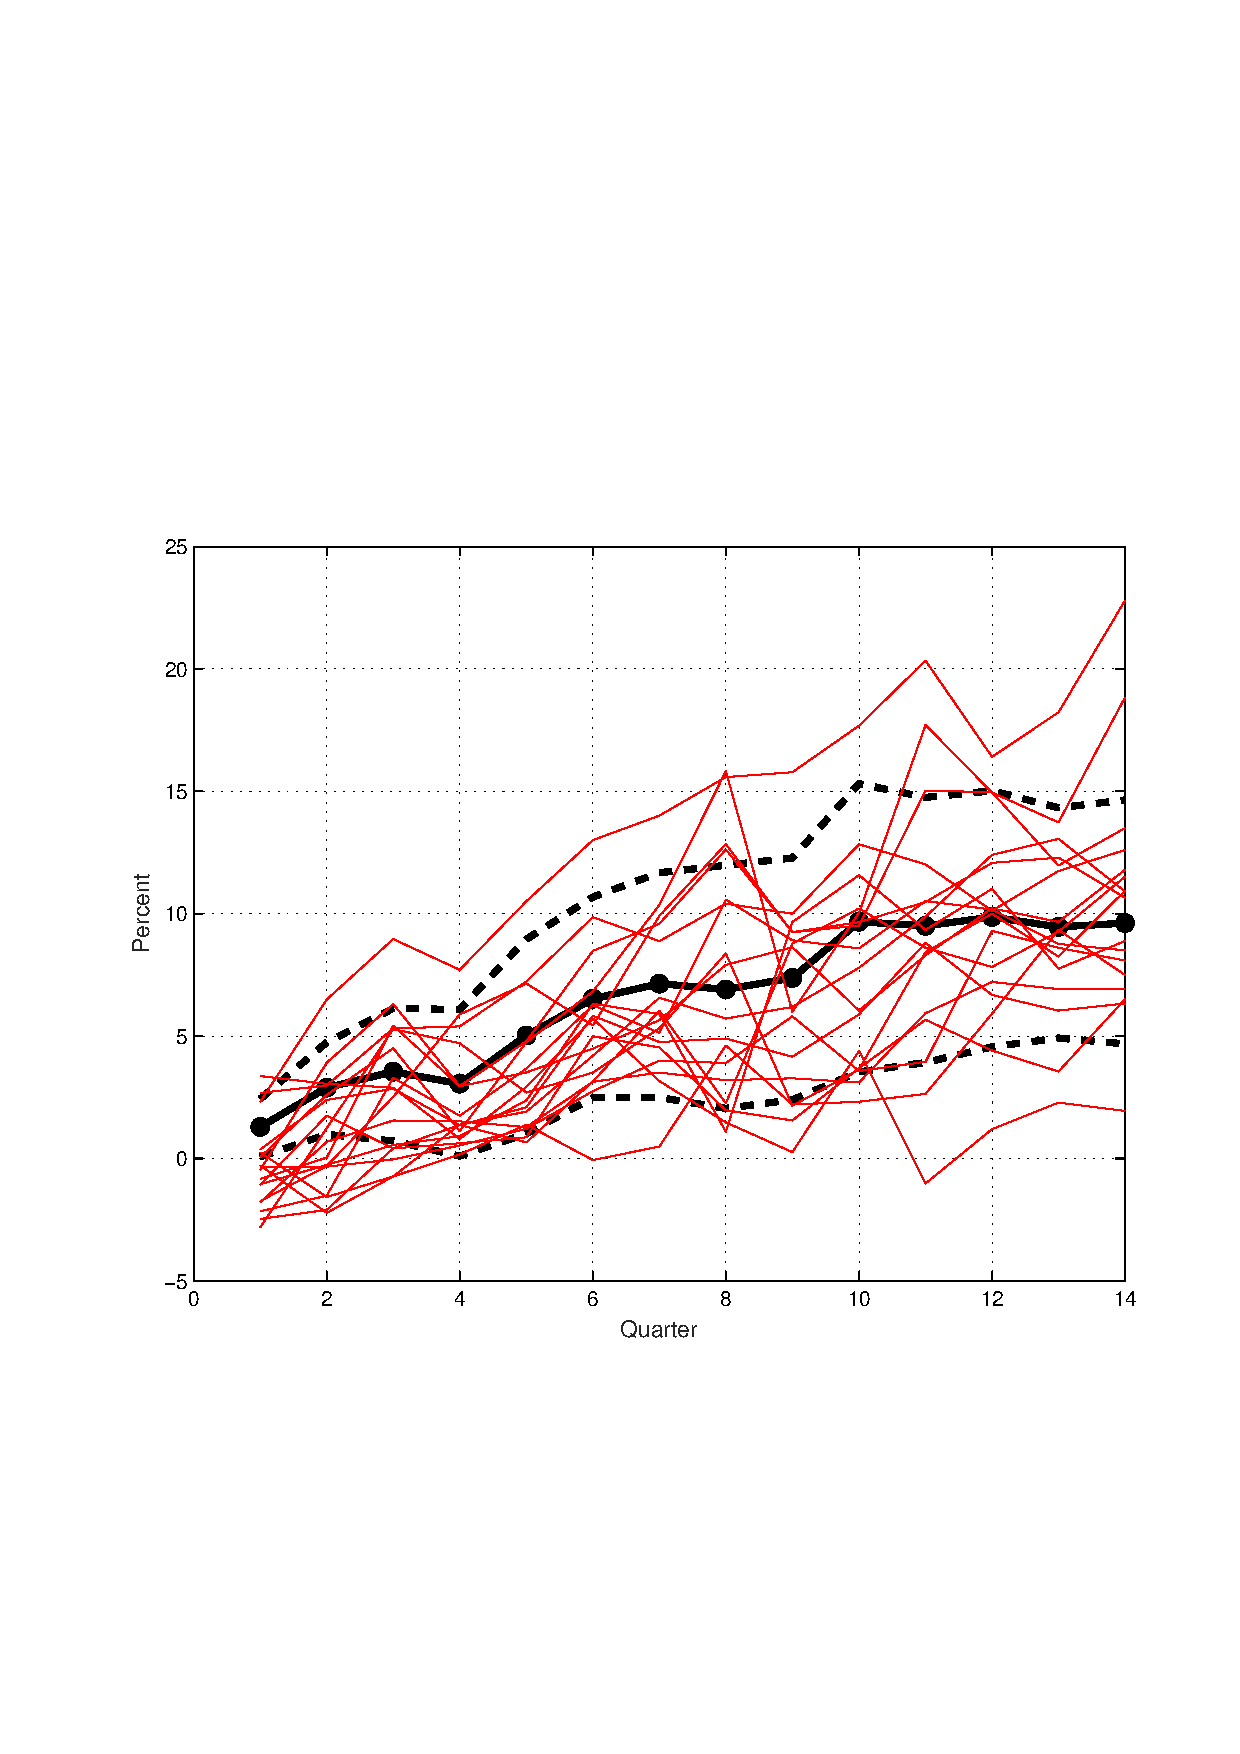
\includegraphics[width=0.7\textwidth]{./figures/fRegHP}\\
%{\scriptsize Numbers in brackets: Initial levels of mean gross Hh income. }
\end{center}
\end{figure}

\end{frame}



\begin{frame}\frametitle{\bf ES regional house prices: IRF vs level \hyperlink{Robust}{\beamergotobutton{Back}} \hypertarget{ESlocalHPlevel}{}}
Positive relationship b/w level and response of HP
\begin{figure}
\begin{center}
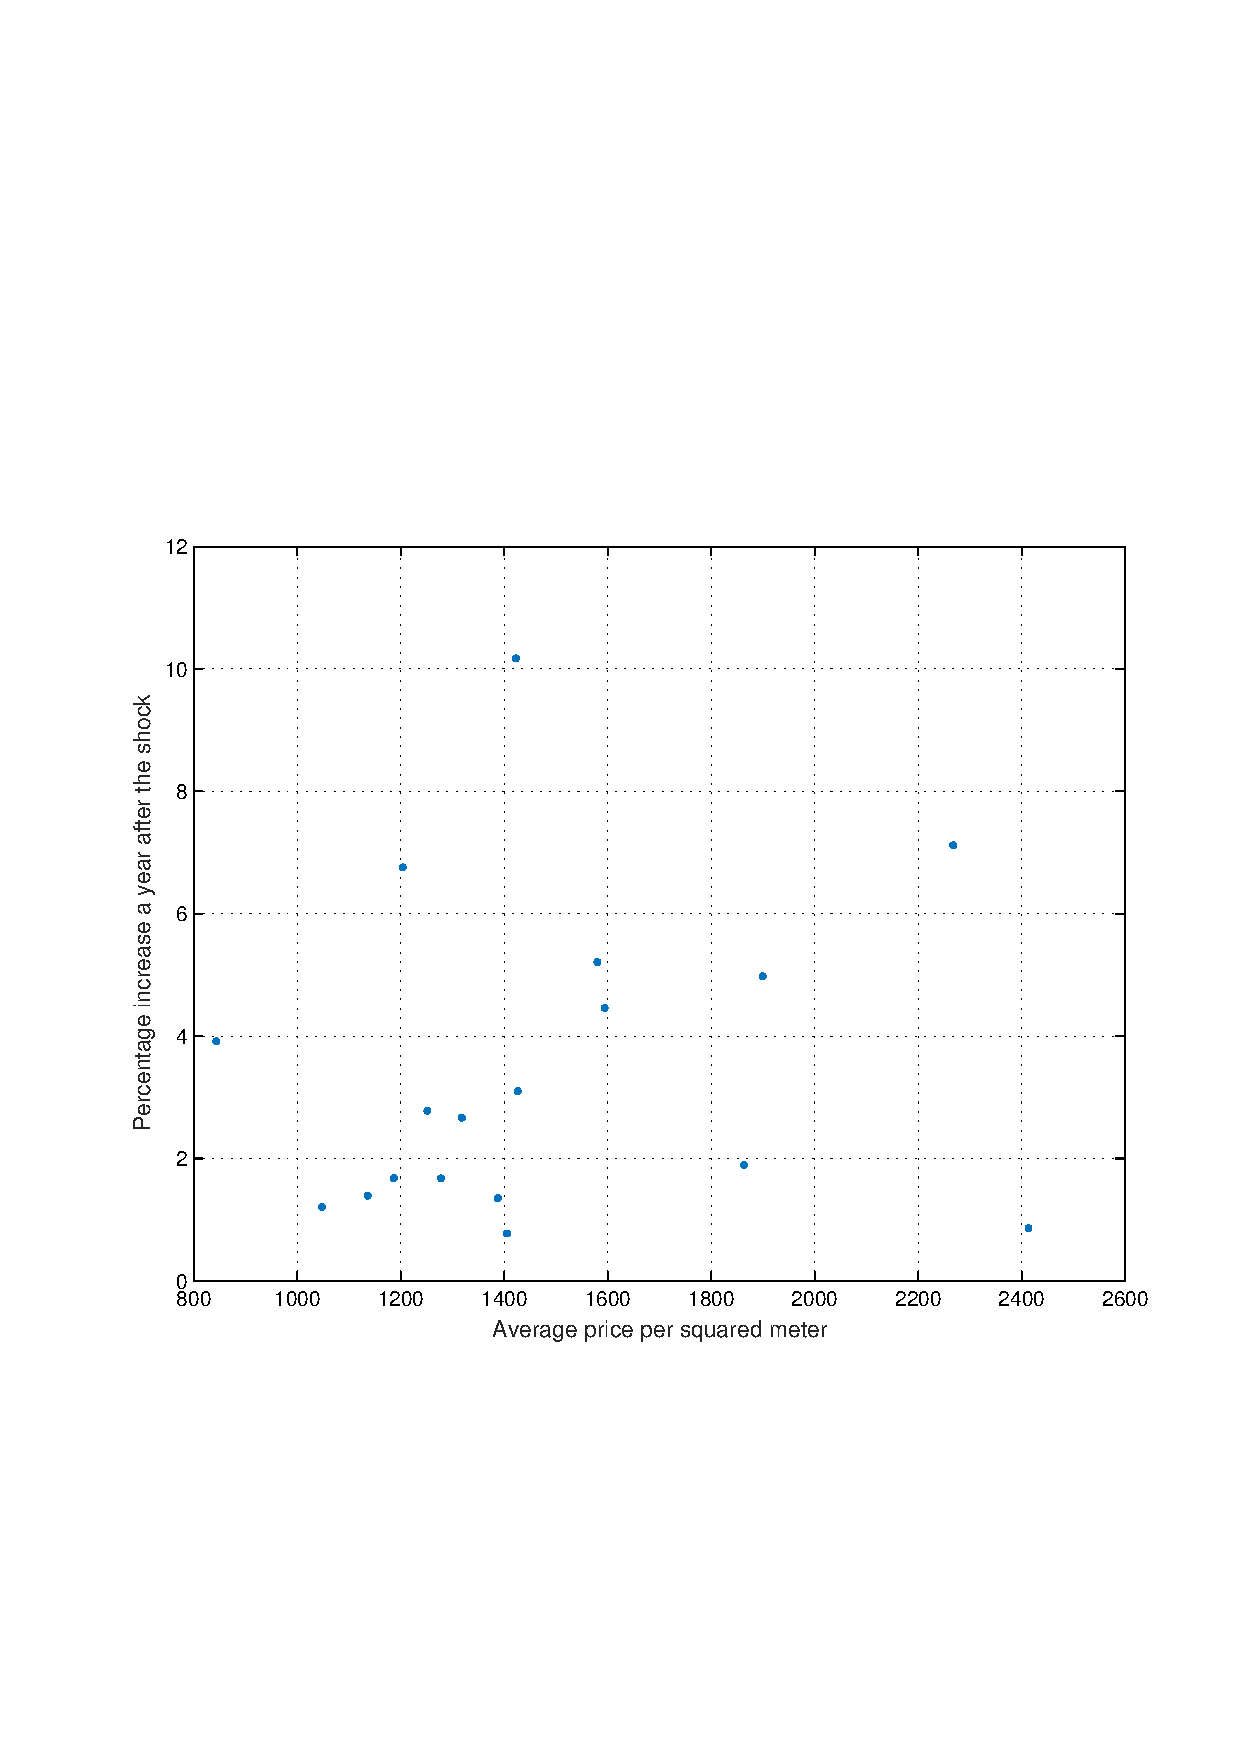
\includegraphics[width=0.7\textwidth]{./figures/fHP_irf_level_scatter}\\
%{\scriptsize Numbers in brackets: Initial levels of mean gross Hh income. }
\end{center}
\end{figure}

\end{frame}


\begin{frame}\frametitle{\bf Local linear projection:   Profits $\uparrow$ by 5\% \hyperlink{Robust}{\beamergotobutton{Back}} \hypertarget{finInc}{}}
%Financial income matters most in the upper tail
\begin{figure}
\begin{center}
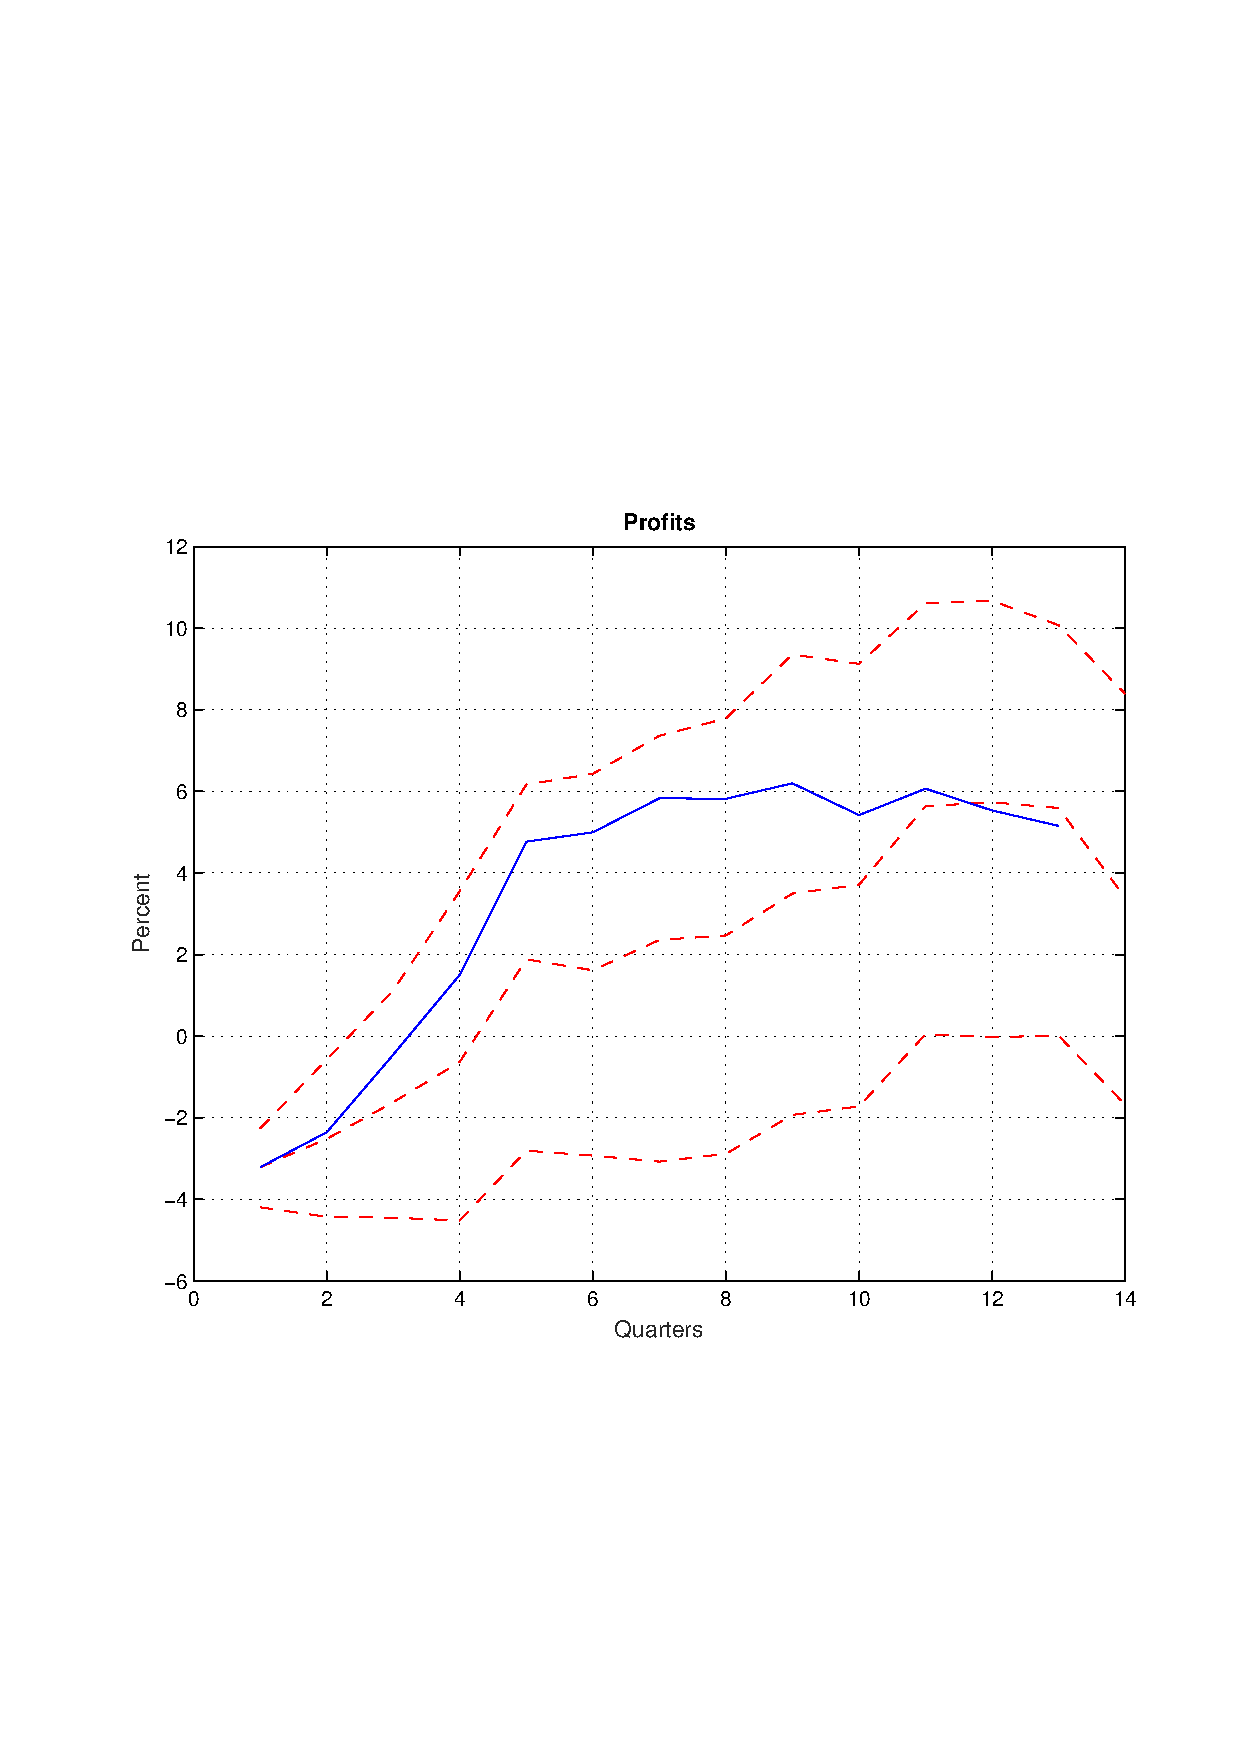
\includegraphics[width=0.7\textwidth]{./figures/fProfits}\\
%{\scriptsize Numbers in brackets: Initial levels of mean gross Hh income. }
\end{center}
\end{figure}

\end{frame}


\begin{frame}\frametitle{\bf Robustness: Uniform employment probability \hypertarget{UniformEmpProb}{}}
{\scriptsize Baseline IRFs (Solid) vs IRFs under uniform probability of getting employed (Dashed) \hyperlink{Robust}{\beamergotobutton{Back}}}

\begin{figure}
\begin{center}
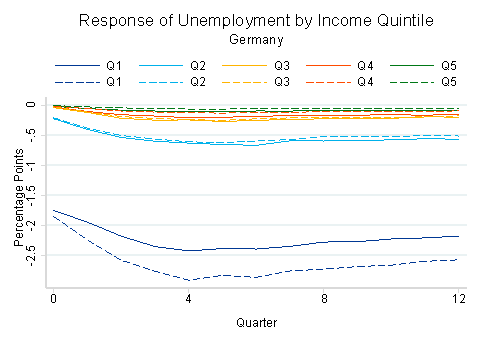
\includegraphics[width=0.40\textwidth]{./figures/UR_chart_DE_compare_uni}
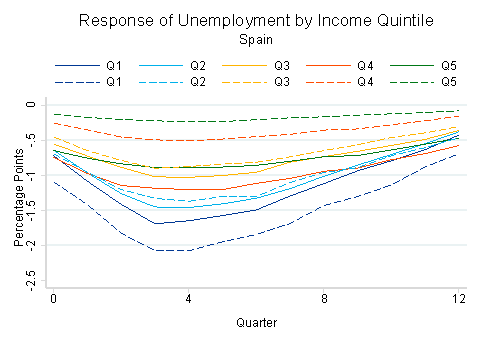
\includegraphics[width=0.40\textwidth]{./figures/UR_chart_ES_compare_uni}\\
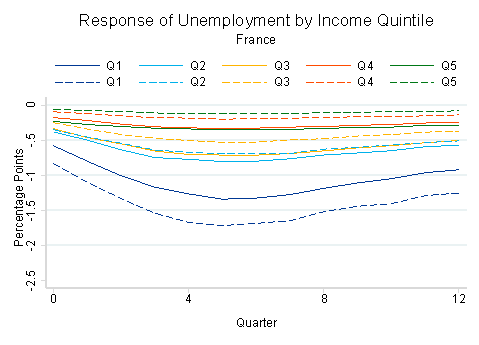
\includegraphics[width=0.40\textwidth]{./figures/UR_chart_FR_compare_uni}
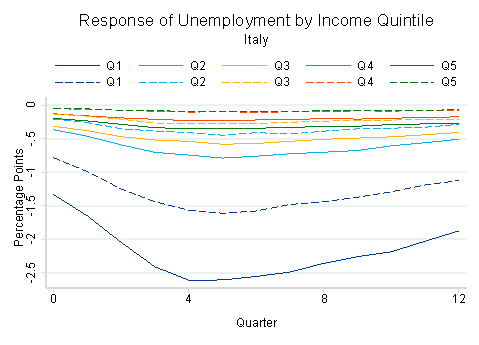
\includegraphics[width=0.40\textwidth]{./figures/UR_chart_IT_compare_uni}
\end{center}
\end{figure}
\end{frame}

\begin{frame}\frametitle{\bf Robustness: Same VAR response in all countries \hypertarget{SameXC}{}}
{\scriptsize Baseline IRFs (Solid) vs IRFs restricted to be the same across countries (Dashed) \hyperlink{Robust}{\beamergotobutton{Back}}}

\begin{figure}
\begin{center}
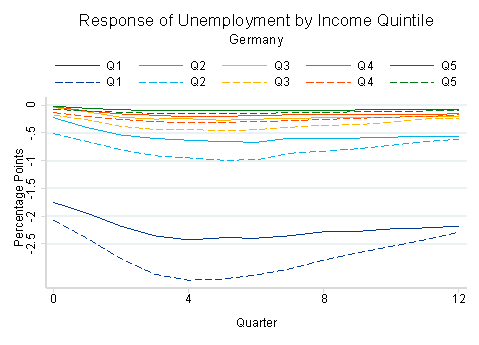
\includegraphics[width=0.40\textwidth]{./figures/UR_chart_DE_compare_noXC}
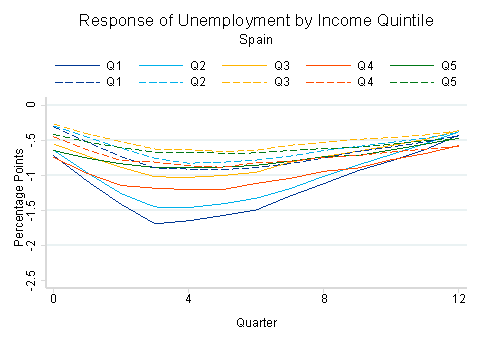
\includegraphics[width=0.40\textwidth]{./figures/UR_chart_ES_compare_noXC}\\
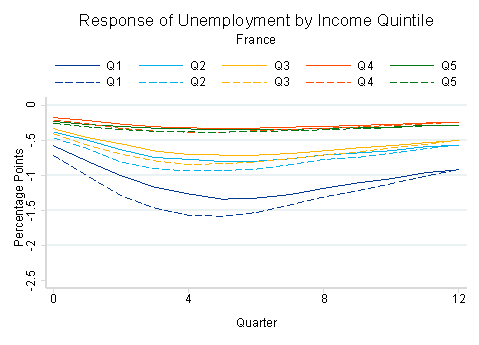
\includegraphics[width=0.40\textwidth]{./figures/UR_chart_FR_compare_noXC}
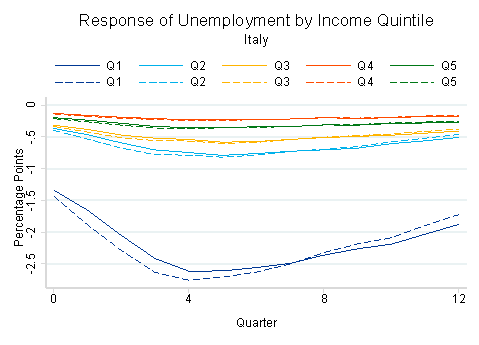
\includegraphics[width=0.40\textwidth]{./figures/UR_chart_IT_compare_noXC}
\end{center}
\end{figure}

\end{frame}


\begin{frame}\frametitle{\bf Robustness: Financial income $\uparrow$ by 5\% \hypertarget{FinInc}{}}
Financial income matters most in the upper tail \hyperlink{Robust}{\beamergotobutton{Back}}
\begin{figure}
\begin{center}
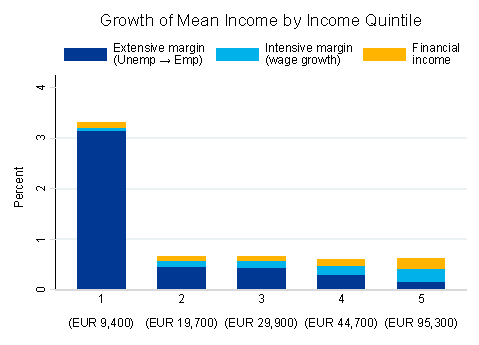
\includegraphics[width=0.7\textwidth]{./figures/meanIncomeByIncQuint_EA_decompFinInc_per4}\\
{\scriptsize Numbers in brackets: Initial levels of mean gross Hh income. }
\end{center}
\end{figure}

\end{frame}


\begin{frame}\frametitle{\bf Robustness: Holdings of stocks $\uparrow$ by 15\% \hypertarget{StockBoost}{}}
Similar overall results \hyperlink{Robust}{\beamergotobutton{Back}}\\
High leverage at the bottom
\begin{figure}
\begin{center}
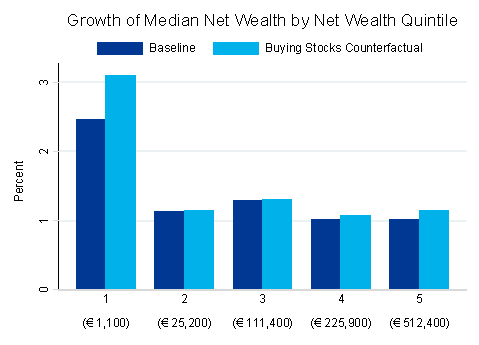
\includegraphics[width=0.7\textwidth]{./figures/medianNetWealthByWquint_EA_stockBoost_15}\\[-2mm]
{\scriptsize Numbers in brackets: Initial levels of median net wealth. }
\end{center}
\end{figure}

\end{frame}



\begin{frame}\frametitle{\bf Net nominal positions}

\begin{figure}
\begin{center}
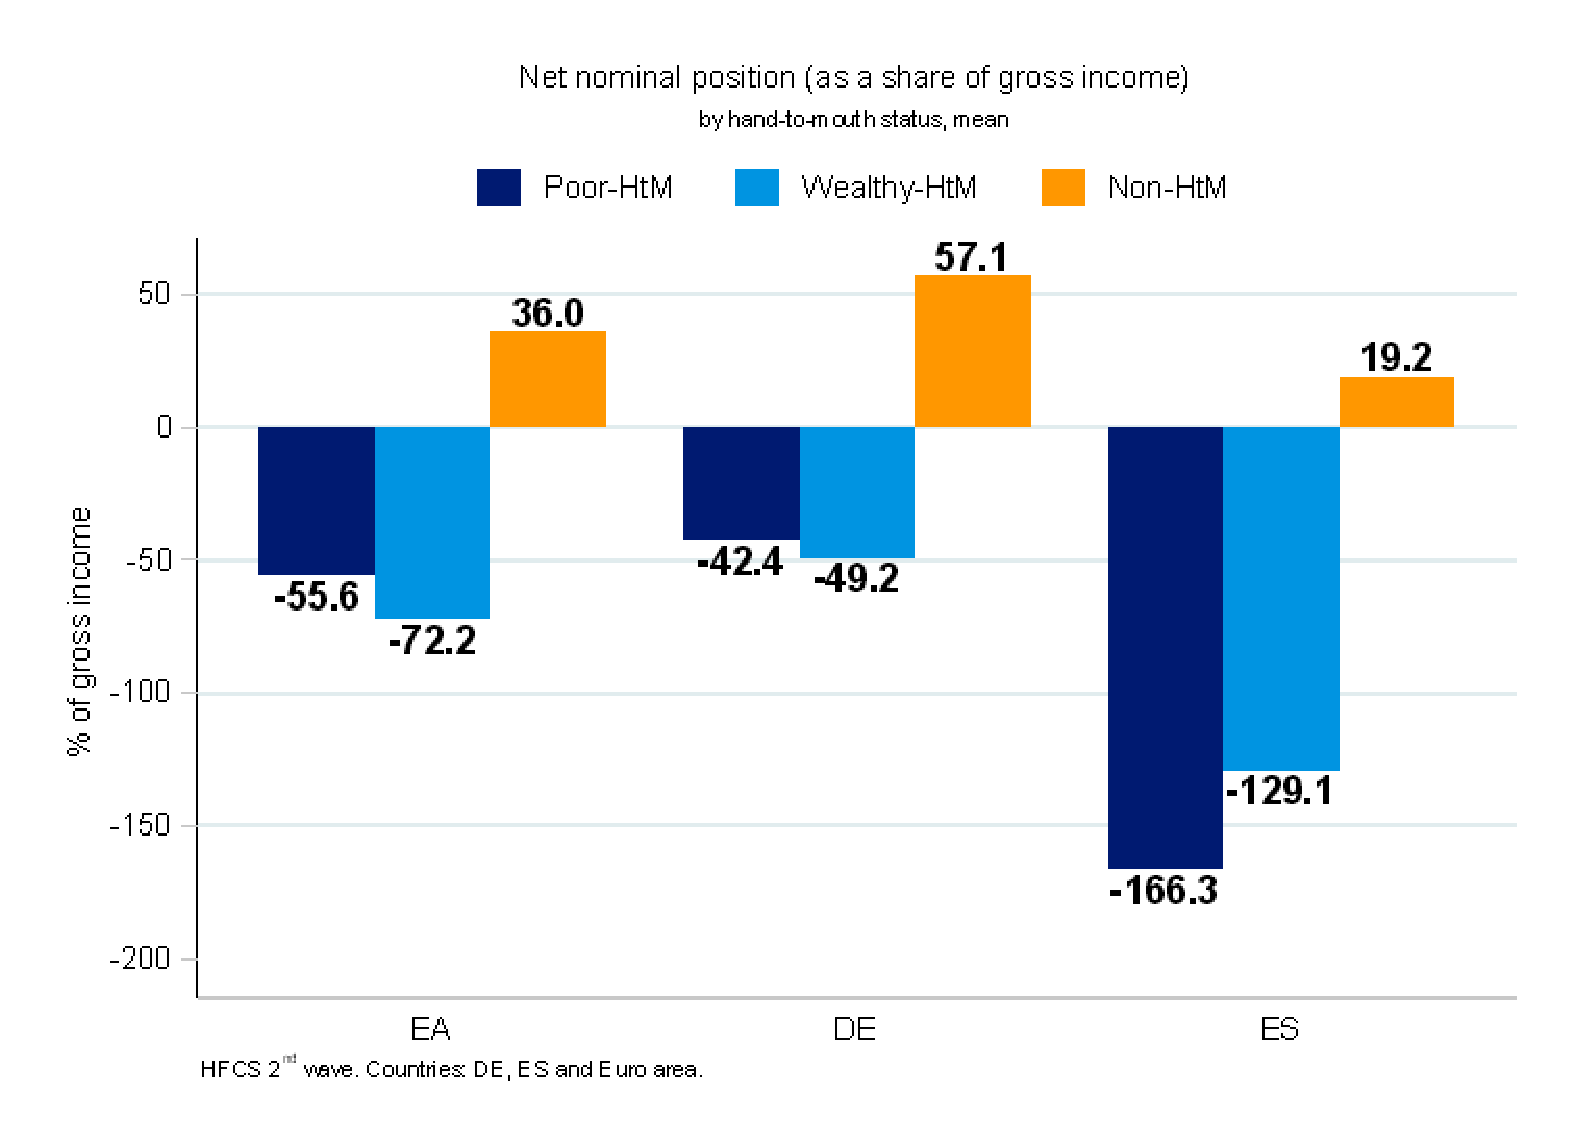
\includegraphics[width=0.8\textwidth]{./figures/NNP.pdf}
\end{center}
\end{figure}

\end{frame}



\begin{frame}\frametitle{\bf Net interest rate exposure---Auclert (2017)}

%\vspace*{-2.5mm}
\footnotesize
\bi
\item Net interest rate exposure = maturing assets - maturing liabilities
\item Maturing assets = 25\%\ of value of mutual funds, bonds, shares, managed accounts, money owed to households, other assets + 100\%\ of deposits
\item Maturing liabilities = 100\%\ outstanding balance of adjustable-rate mortgages + 100\%\ outstanding balance of other non-collateralized debt
\ei
\begin{figure}
\begin{center}
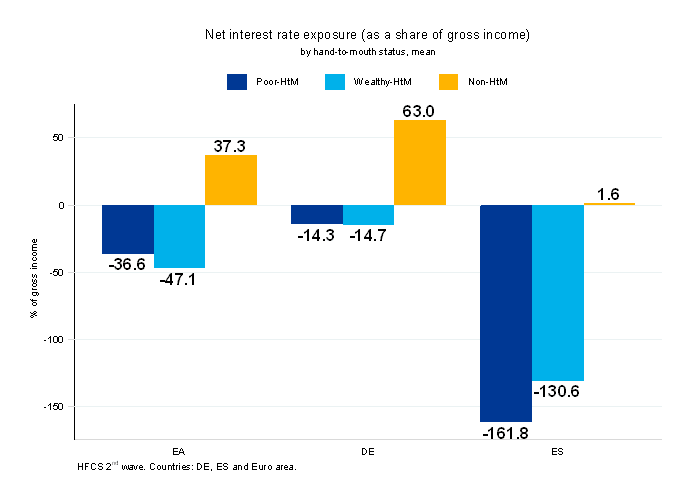
\includegraphics[width=0.6\textwidth]{./figures/netIRexposure.png}
\end{center}
\end{figure}
\end{frame}



\begin{frame}\frametitle{\bf Nonstandard vs Standard MP}


\bi
\item Targeting the same peak GDP response, VAR gives:\\ \jemph{30 bp change in term spread ${}\approx{}$ 100 bp change in policy rate}
\item BUT also qualitative differences (ZLB, differential effects on prices of specific assets, \dots)
\ei
%\bi
%\item More robustness, eg alternative VAR identifications
%\item Accounting for financial income
%\item Wealth: Modeling portfolio rebalancing (?)
%\ei

\end{frame}



%-----------------------------------------------------------------------
%%%%%%%%%%%%%%%%%%%%%%%%%%%%%%%%%%%



%\begin{frame}
%\frametitle{\bf References}
%\end{frame}

\end{document}
